\documentclass[a4paper, 12pt, twoside]{report} 
\usepackage[english]{babel}
\usepackage[utf8]{inputenc}
\usepackage[acronym, toc]{glossaries}
\usepackage{comment}
\usepackage{nomencl}
\usepackage{xargs}                      % Use more than one optional parameter in new commands
\usepackage[pdftex, dvipsnames]{xcolor}  % Coloured text etc.
\usepackage[colorinlistoftodos, prependcaption, textsize=tiny]{todonotes}
\usepackage{amsthm}
\usepackage{amssymb}
\usepackage{graphicx}
\usepackage{siunitx}
\usepackage{booktabs}
\usepackage{hyperref}
\usepackage{pdfsync}
\usepackage{minted}
\usemintedstyle{manni}
\usepackage{listings}
\usepackage{xcolor}
\graphicspath{{./images/}}
\synctex=1

\newcommandx{\unsure}[2][1=]{\todo[linecolor=red, backgroundcolor=red!25, bordercolor=red, #1]{#2}}
\newcommandx{\change}[2][1=]{\todo[linecolor=blue, backgroundcolor=blue!25, bordercolor=blue, #1]{#2}}
\newcommandx{\info}[2][1=]{\todo[linecolor=OliveGreen, backgroundcolor=OliveGreen!25, bordercolor=OliveGreen, #1]{#2}}
\newcommandx{\improvement}[2][1=]{\todo[linecolor=Plum, backgroundcolor=Plum!25, bordercolor=Plum, #1]{#2}}
\newcommandx{\thiswillnotshow}[2][1=]{\todo[disable, #1]{#2}}

\newtheorem{parameter}{Parameter%}
%
% background color
%\pagecolor{black}
%\color{white}

% glossaries
\makeglossaries

\newacronym{abm}{ABM}{Agent-Based Models}
\newacronym{act}{ACT}{artemisinin-based combination therapy}
\newacronym{auc}{AUC}{Area under curve}
\newacronym{bmgf}{BMGF}{Bill & Melinda Gates Foundation}
\newacronym{cea}{CEA}{cost-effectiveness analysis}
\newacronym{eht}{EHT}{Experimental Hut Trial}
\newacronym{gdg}{GDG}{guideline development group}
\newacronym{hbi}{HBI}{Human Blood Index}
\newacronym{icers}{ICERs}{Incremental cost-effectiveness ratios}
\newacronym{irs}{IRS}{Indoor Residual Spraying}
\newacronym{itn}{ITN}{Insecticide Treated Nets}
\newacronym{llins}{LLINs}{Long Lasting Insecticide Treated Nets}
\newacronym{mcmc}{MCMC}{Markov Chain Monte Carlo}
\newacronym{mda}{MDA}{mass drug administration}
\newacronym{msat}{MSAT}{mass screening, and treatment approach}
\newacronym{nmcp}{NMCP}{National Malaria Control Programme}
\newacronym{odd}{ODD}{overview, design concepts, and details}
\newacronym{pamca}{PAMCA}{Pan-African Mosquito Control Association}
\newacronym{pbo}{PBO}{piperonyl, butuxide}
\newacronym{pfpr}{\textit{Pf}PR}{\textit{Plasmodium falciparum} parasite rate}
\newacronym{pvprlm}{\textit{Pv}{PR}$_{LM}$}{parasite prevalence by light microscopy}
\newacronym{rct}{RCT}{Clustered Randomized Control Trial}
\newacronym{ssa}{SSA}{sub-Saharan Africa}
\newacronym{smc}{SMC}{Seasonal Malaria Chemoprevention}
\newacronym{vbd}{VBD}{vector borne diseases}

\newglossaryentry{xgboost}
{name={XGBoost},
  description={Extreme Gradient boosting, popularly referred to as XGBoost, is a machine learning method that is used to solve regression, and classification problems. It provides results in a prediction model, mostly in the form of trees. It is scalable, and efficient in memory usage, and drives fast learning through parallel, and distributed computing.}
}

\newglossaryentry{foi}
{name={force of infection},
  description={force of infection from human to mosquito, and from mosquito to human}
}
\newglossaryentry{dalys}
{name=DALYs,
  description={Disability Adjusted Life Years. The sum of years of potential life lost due to premature mortality, and the years of productive life lost due to disability.}
}
\newglossaryentry{endophilic}
{name=endophilic,
  description={indoor-resting}
}
\newglossaryentry{exophilic}
{name=exophilic,
  description={outdoor-resting}
}
\newglossaryentry{exphagic}
{name=exphagic,
  description={outdoor-biting}
}
\newglossaryentry{zoophagic}
{name=zoophagic,
  description={blood feeding not only from human }
}

\newglossaryentry{carbamates}
{name=carbamates,
  description={Carbamates are a class of insecticides structurally, and mechanistically similar to organophosphate (OP) insecticides. Carbamates are N-methyl Carbamates derived from a carbamic acid, and cause carbamylation of acetylcholinesterase at neuronal synapses, and neuromuscular junctions.}
}

\newglossaryentry{bendiocarb}
{name=bendiocarb,
  description={Bendiocarb is an acutely toxic carbamate insecticide used in public health, and agriculture, and is effective against a wide range of nuisances, and disease vector insects. Many bendiocarb products are or were sold under the tradenames `Ficam', and `Turcam.'}
}

\newglossaryentry{carbosulfan}
{name=carbosulfan,
  description={Carbosulfan is an organic compound adherent to the carbamate class. At normal conditions, it is brown viscous liquid. It is not very stable; it decomposes slowly at room temperature. Its solubility in water is low, but it is miscible with xylene, hexane, chloroform, dichloromethane, methanol, and acetone.}
}

\newglossaryentry{IRAC MoA}
{name=IRAC MoA,
  description={The IRAC MoA classification scheme covers more than 25 different modes of action, and at least 55 different chemical classes. Diversity is the spice of resistance management by chemical means, and thus it provides an approach to IRM providing a straightforward means to identify potential rotation/alternation options.}
}

\newglossaryentry{IVCC}
{name=IVCC,
  description={IVCC is the only Product Development Partnership (PDP) working in vector control. IVCC was established in 2005, through an initial \$50million grant to the Liverpool School of Tropical Medicine (LSTM) from the Bill & Melinda Gates Foundation, and is a registered charity in the UK\@. We work with stakeholders to facilitate the development of novel, and improved public health insecticides, and formulations to combat the rapidly growing problem of insecticide resistance. We bring together partners from industry, the public sector, and academia to create new solutions to prevent disease transmission. By focusing resources, and targeting practical scientific solutions we accelerate the process from innovation to impact.}
}

\newglossaryentry{rts}
{name=RTS\,S,
	description={RTS\,S/AS01 is a recombinant protein-based malaria vaccine.}
}

\newglossaryentry{eir}
{name=EIR,
	description={Entomological Infectious Rate or infected bites per person per year}
}

\newglossaryentry{eip}
{name=extrinsic incubation period,
  description={Once ingested by a mosquito, malaria parasites must undergo development within the mosquito before they are infectious to humans. The time required for development in the mosquito (the extrinsic incubation period) takes 9 days or longer, depending on the parasite species, and the temperature.}
}

\newglossaryentry{isc}
{name=intra-specific competition,
  description={Intraspecific competition is an interaction in population ecology, whereby members of the same species compete for limited resources. This leads to a reduction in fitness for both individuals, but the most fit individual survives, and is able to reproduce. By contrast, interspecific competition occurs when members of different species compete for a shared resource.}
}

\newglossaryentry{R0}
{
  name=R0,
  description={In epidemiology, the basic reproduction number, or basic reproductive number (sometimes called basic reproduction ratio or basic reproductive rate), denoted $R_0$ (pronounced R nought or R zero), of an infection is the expected number of cases directly generated by one case in a population where all individuals are susceptible to infection.}
}

% nomenclature
\makenomenclature

%\nomenclature{$c$}{Speed of light in a vacuum inertial frame}

% title page
\title{An Overview of Malaria Mathematical Modeling}
\author{Chunzhe ZHANG}
\date{2021}

\begin{document}

\begin{titlepage}
	\maketitle
\end{titlepage}

\tableofcontents

\printglossaries
\printnomenclature

\newpage
\chapter{Introduction}
Mathematical modeling is a vital way to help public health practitioners to make policy decisions.
Mathematical models have been introduced into the malaria control world for many years.
History could go back to 1911, Christophers\cite{christophers1911epidemic} developed an early-warning system for malaria epidemics with rainfall, fever-related deaths, and wheat prices.
Then in the 1920s, Ronald Ross introduced the famous version of the Ross-McDonald model.
In the 1970s, model simulations were compared to field observations to estimate the parameter values giving the best fit possible, and evaluate the model by analyzing the discrepancies between the observed, and expected values\cite{dietz1974}.
Model\cite{Weiss2020e} was applied to understand the potential indirect effects of the COVID-19 pandemic on malaria intervention coverage, morbidity, and mortality.
Mathematical models could also apply to understand the progression of the disease.
The interaction between red blood cells, merozoites, and platelets during malaria infection was modeled mathematically\cite{Alves2021} to understand platelets' role in antiparasitic action.

The substantial decade-long reduction in global malaria burden stalled in 2016 with an estimated increase of 5 million cases.
Modeling suggests 70\% of the reduction in malaria cases in \gls{ssa} between 2000, and 2015 was attributable to implementing intervention strategies.
Critical interventions included \gls{itn}, \gls{act}, and \gls{irs}.
Models use field data as evidence for the efficacy, and cost-effectiveness of selected interventions; however, these methods can be resource-intensive or have prohibitive ethical barriers.
In such situations, mathematical simulation is increasingly beneficial to provide further insights.

The most valuable modeling information for policy-makers is on the effectiveness, and cost-effectiveness of malaria interventions, and their combinations in different settings, in reducing transmission, morbidity, and mortality, and in potentially interrupting transmission.

Modeling can help answer questions as:

\begin{itemize}
	\item What combination of interventions would achieve the highest impact given fixed resources?
	\item In low-transmission settings, what combination of interventions or changes can help interrupt transmission?
	\item What is the optimal coverage of specific intervention? Is it beneficial to add a second vector control intervention to a population with already high coverage of one intervention?
\end{itemize}

At the \gls{nmcp} level, modeling could help set up precise criteria on WHO recommendations to create a transition from policy-making to planning.
For malaria control product research and development planners, models could help devise target product profiles for new interventions requiring minimum efficacy and durability of an intervention.

However, differences in model methods, structures, and data being used in parameter calibration result in no consensus yet exists on model's optimal version or output.
Conflicts in the different model predictions arise from the data sets used in their calibration, and the behind mechanism.
Thus, we must know how modeler assemble the model, and the assumptions on which they are built.

\chapter{Mathematical Methods}

%\paragraph{Differences of two models}%
%\label{par:differences_of_two_models}

%\begin{table}[ht]
%	\centering
%	\label{tab:difference}
%	\begin{tabular}{c c c}
%		\toprule
%		                      & Deterministic                & Stochastic                          \\
%		\midrule
%		Immunity Level        & An average level for a group & Different level for each individual \\
%		Fitting to Real World & Easy                         & Complex                             \\
%		\bottomrule
%	\end{tabular}
%	\caption{Difference of Deterministic, and Stochastic Model}
%\end{table}

\section{The Relationships and Differences between Deterministic, Stochastic, and Compartmental Models}
`Deterministic, stochastic, and compartmental' are the three most prevailing terminologies in malaria mathematic modeling.
To gain a better insight into mathematical modeling, awareness of these concepts is a prerequisite.

\subsection{Compartmental Models}%
\label{subsubsec:compartmental}
\textbf{Compartment}, or alcove, cell, chamber, is a nomenclature for grouping an assemblage of individuals into same clusters.
Compartmental models describe a dynamic system with finite chambers.
Each connects one or more chambers.
In epidemiology, compartmental modeling involves stratifying the population with multiple compartments, such as susceptible, treatment, isolation, and exposure.
Models then further focus on interactions and transitions between population strata, and have been a mainstay of modeling in such areas for more than a century.

Compartmental models simplify the mathematical modeling of infectious diseases.
Models assign the population to compartments with labels – for example, S, I, or R(Susceptible, Infectious, or Recovered).
The labels' order usually shows the flow patterns between the compartments; for example, \textbf{SEIS} means susceptible, exposed, infectious, then susceptible again.

\subsubsection{SIR Models}
SIR models are a group of fundamental compartmental models.
These models focus on describing the dynamics of human infectious states.
Variations of SIR models include:

\subsubsection{SI Model}
The first effort of introducing compartmental models into epidemiology is to separate the population into $S$, and $I$ compartment.
Here, $S$ stands for the susceptible population, and $I$ stands for infected population.

The SI model assumes a constant rate of the recovery rate of the infection group.
\begin{align}
	\frac{dS}{dt} & = - \lambda S \\
	\frac{dI}{dt} & = \lambda S
\end{align}

\begin{center}
$\lambda$ -  \gls{foi}\\
\end{center}

\begin{figure}[htpb]
	\centering
	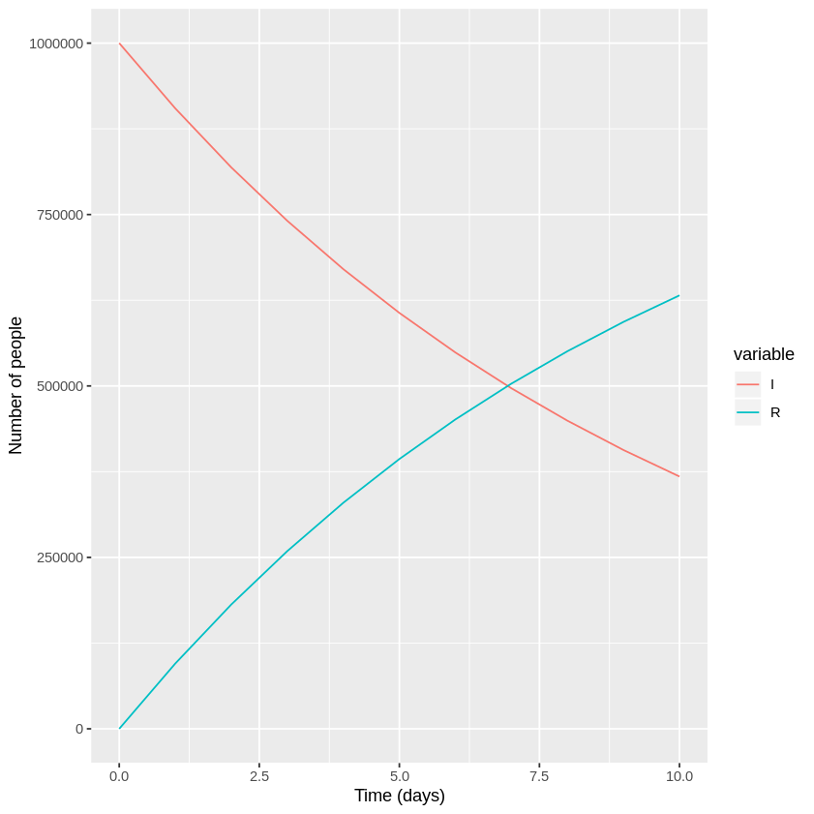
\includegraphics[width=0.8\textwidth]{si-model}
	\caption{A Simulation of SI Model}
	\label{fig:si-model}
\end{figure}

\subsubsection{SIR Model}
SIR model is the most fundamental infectious disease compartmental model by introducing another chamber called $R$, which stands for the recovery population.
\begin{align}
	\frac{dS}{dt} & = - \lambda S          \\
	\frac{dI}{dt} & = \lambda S - \gamma I \\
	\frac{dR}{dt} & = \gamma I
\end{align}
\begin{center}
$\gamma$ - recovery rate \\
\end{center}

\begin{figure}[htpb]
	\centering
	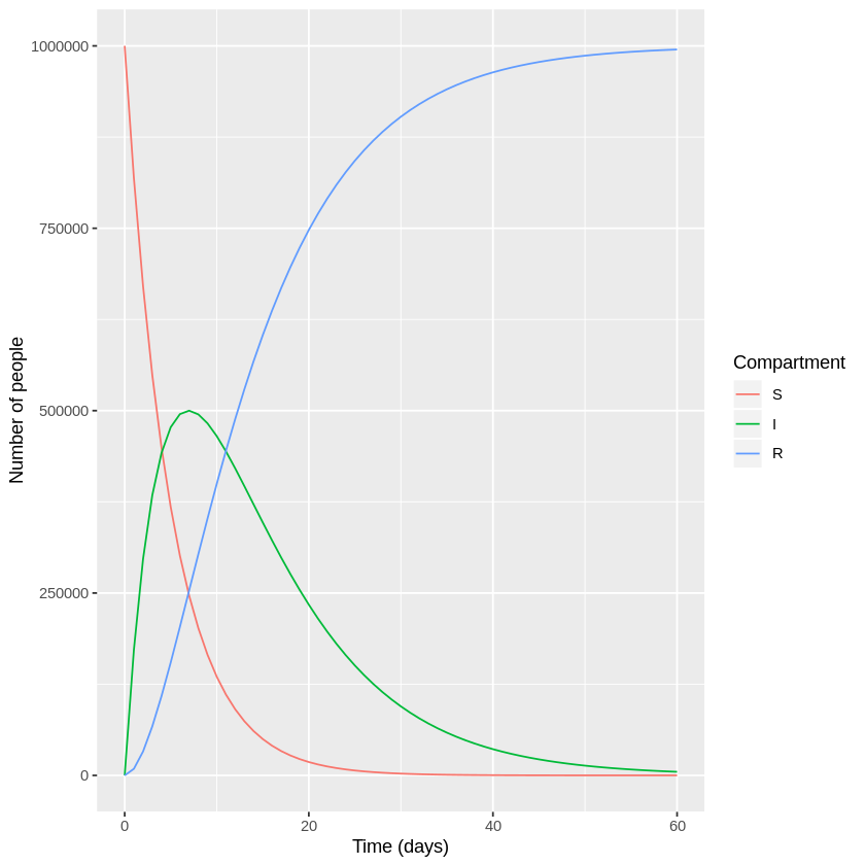
\includegraphics[width=0.8\textwidth]{sir-model}
	\caption{A Simulation of SIR Model}
	\label{fig:sir-model}
\end{figure}

The periods from start to end of epidemics are often too fast to include birth and death dynamics.
Therefore, birth and death are often omitted in simple compartmental models.
However, to reproduce for a further extended duration, such as in malaria control, birth and death could not be excluded.
The birth and death rate will reconstruct the population age structure, and influence the overall immunity against \textit{Plasmodium}.

The extension of SIR model including birth and death rate:
\begin{equation}
  \frac{dS}{dt}=-\lambda S-\mu S+bN
\end{equation} 
\begin{center}
  b - birth rate \\
  $\mu$ - death rate \\
\end{center}  

In the above setting, $\lambda$ or  \gls{foi} is considered constant.
Nevertheless, this does not abide by real-world scenarios in which the \gls{foi} will drop down as the susceptible population runs out.
In this setting, the $\lambda$ in SIR model was further extended to be dynamic.
\begin{equation}
	\lambda = \beta \frac{I}{N}
\end{equation}

$\beta$ is the infection rate, and $N$ is the total population.
Studies explored different combinations of $\beta$, and $\gamma$, and the ratio between these two fundamental parameters forms the first idea of \gls{R0}.
\begin{equation}
	R_0 = \frac{\beta}{\gamma}
\end{equation}
\begin{figure}[htpb]
	\centering
	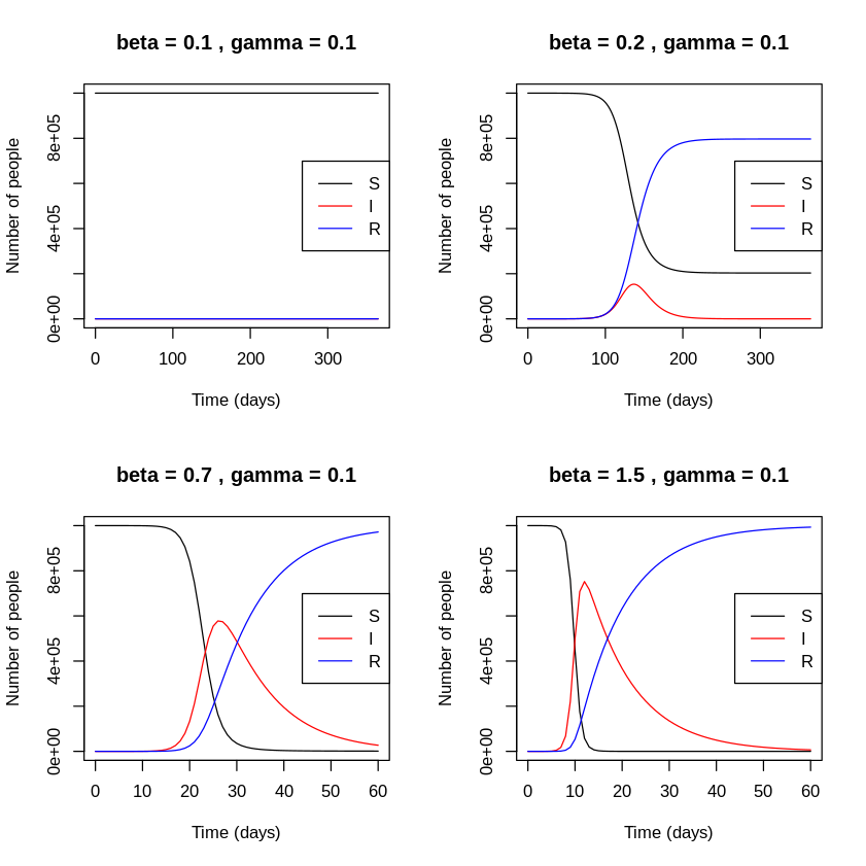
\includegraphics[width=0.8\textwidth]{sir-model-beta-gamma}
	\caption{Comparison of combination of $\beta$, and $\gamma$}
	\label{fig:sir-model-beta-gamma}
\end{figure}

By definition, if $\beta > \gamma$, the epidemic will take off, and vice versa.
However, the definition of \gls{R0} changes accordingly with the different model.
For example, if the SIR model separates infection group into symptomatic, and asymptomatic infection groups.
\begin{figure}[htpb]
	\centering
	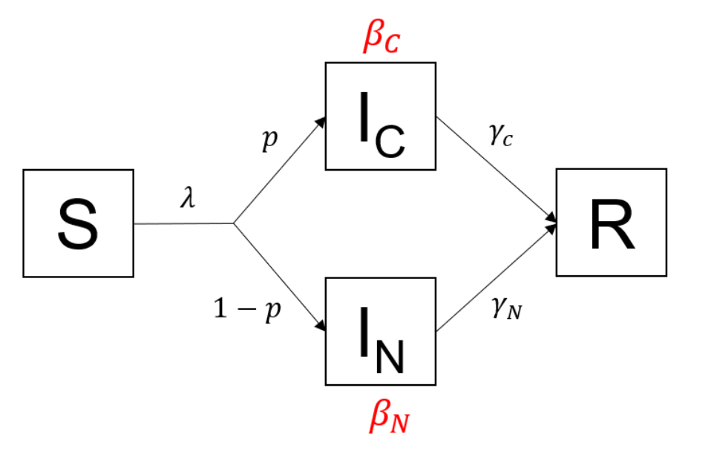
\includegraphics[width=0.8\textwidth]{sir-model-asymptomatic}
	\caption{SIR model structure with asymptomatic compartment}
	\label{fig:sir_model_structure_with_asymptomatic_compartment}
\end{figure}

The calculation of \gls{R0} will change to:
\begin{equation}
	R_0 = p \frac{\beta_c}{\gamma_c} + (1-p) \frac{\beta_N}{\gamma_N}
\end{equation}

Studies further extend the SIR model to model population turnover, and waning immunity against some diseases.
For example, by incorporating the birth and death effect in the model, the number of infected people oscillates over time.
\begin{align}
	\frac{dS}{dt} & = - \lambda S - \mu S + bN     \\
	\frac{dI}{dt} & = \lambda S - \gamma I - \mu I \\
	\frac{dR}{dt} & = \gamma I - \mu R
\end{align}
\begin{center}
	$\mu$ - the mortality rate of each group, and \\
	$b$ - the birth rate of total population \\
\end{center}

\begin{figure}[htpb]
	\centering
	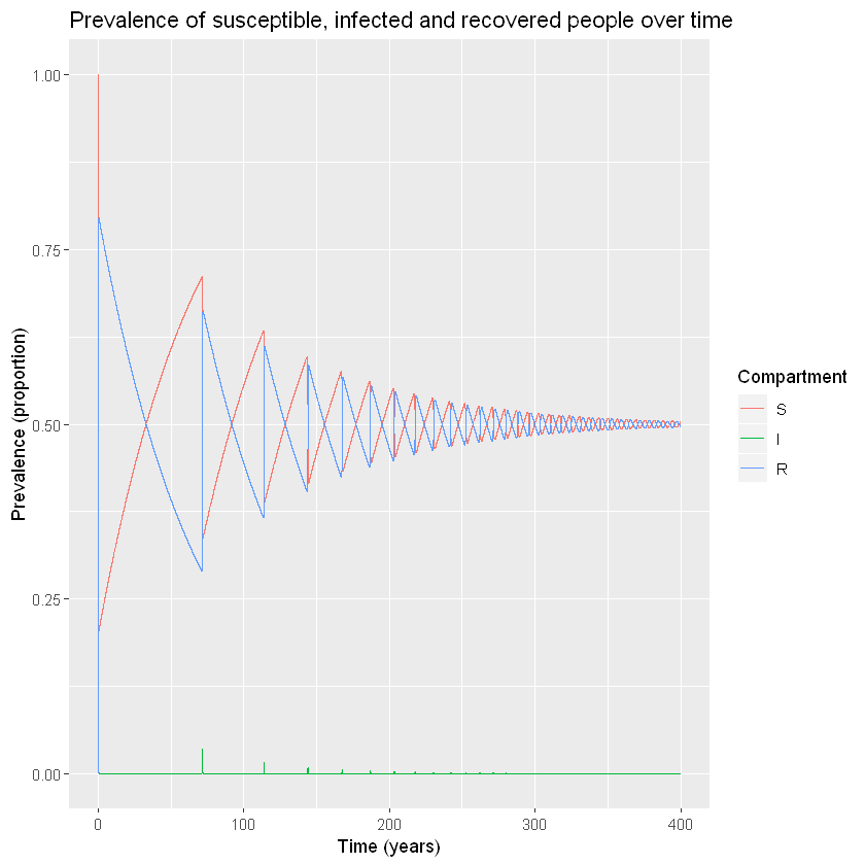
\includegraphics[width=0.8\textwidth]{sir-model-birth-death}
	\caption{SIR Model Simulation with birth and death}
	\label{fig:sir-model-birth-death}
\end{figure}

These sharp epidemic cycles indicate that epidemics repeatedly reoccur over time, although the peaks become progressively smaller, and eventually disappear.
The first peak is the one we looked at above.
This pattern occurs because the disease has a much shorter duration than the human population turnover.
Once an epidemic has spread through the population, and depleted the susceptible pool, it takes a long time for the susceptible to replenish through births.
This is why we see these deep, and long troughs (around 70 years until the second epidemic) between epidemics.

\subsubsection{SEIR Model}
Another extension of SIR model is the SEIR model.
When a pathogen emerges in a host community, it partitions individuals into categories depending on parasite density inside them.
Studies separated $I$ (infection) group into:
\begin{itemize}
  \item The exposed (E) group - the fraction of population whose individuals are already infected, but not capable of transmitting the infection to others within a latent period.
  \item The next is infectious (I) group who could cause more infected individuals through interaction with the S group.
\end{itemize}
Studies further extend the susceptible(S) group's definition to include the fraction of host population that do not have immunity to the disease though they might be infected before.
Those who removed from the infection, either because mortality or recovered, make up the R class. For those recovered from the disease, the immunity level wanes over time, they will move to the S group again.
There are variations in the compartment structure depending on the type of disease.
For example, the I class of individuals may not recover at all, and die; R can consist of individuals, who recover with temporary or permanent immunity, thereby further partitioning the epidemiological compartments.

\subsubsection{\gls{vbd} Model}
Developed more than 70 years ago, Ross-McDonald model is the most fundamental vector borne disease compartmental model.
It was a part of a set of theories for the dynamics of mosquito-transmitted diseases.
The model extends the SEIR model with vector components.
Vectors were separated into susceptible, and infectious group.
The model then linked the human compartments with vector compartments by the biting rate, probability of infection from human to mosquito, and from mosquito to human.
Detailed implementation was described as follow mathematical formulations:

\begin{figure}[htpb]
	\centering
	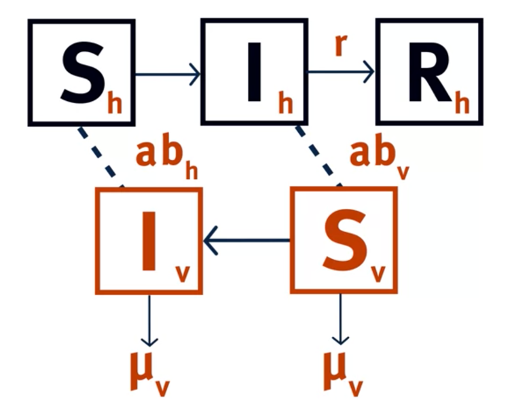
\includegraphics[width=0.8\textwidth]{ross-mcdonald}
	\caption{Ross-McDonald Model Structure}
	\label{fig:ross-mcdonald}
\end{figure}

\begin{align}
	\frac{{dS}_v}{dt} & = \mu_v N_v - ab_vS_v\frac{I_h}{N_h} - \mu_v S_v \\
	\frac{{dI}_v}{dt} & =\ ab_vS_v\frac{I_h}{N_h}-\mu_v I_v              \\
	\frac{{dS}_h}{dt} & =\ -\frac{ab_h}{N_h}S_hI_v                       \\
	\frac{{dI}_h}{dt} & =\ \frac{ab_h}{N_h}S_hI_v-{\rm rI}_h             \\
	\frac{{dR}_h}{dt} & =\ {\rm rI}_h
\end{align}
Where,
\begin{centering}
	$S_v$ - Susceptible Vector  \\
	$I_v$ - Infected Vector\\
	$S_h$ - Susceptible Host\\
	$I_h$ - infected\ host\\
	$R_h$ – recovered host\\
	$\alpha$ - biting rate \\
	$b_v$ – Probability of infection from an infected host to a susceptible vector\\
	$b_h$ – Probability of infection from an infected vector to a susceptible host
\end{centering}

Ross-McDonald further developed the concept of vector capacity, methods for measuring key components of vector disease transmission.
Since then, more versions of \gls{vbd} models emerged based this version.

\subsubsection{Vectorial capacity}
\label{par:interpretation_of_vectorial_capacity_equation}
Ross-McDonald theories derive a concept called vectorial capacity.
It is the index of malaria transmission intensity, or the number of secondary cases arising per day from a single infective case in a susceptible human population.

The following equation defines vectorial capacity:
\begin{equation}
	V\ =\ \frac{ma^2p^n}{-\ln{\left(p\right)}}
\end{equation}

\begin{centering}
	$m$ – ratio vector to human\\
	$a$ – vector human biting rates\\
	$p$	– probability mosquito survive throughout one day\\
	$n$	–	\gls{eip}
\end{centering}

Multiple studies\cite{LeMenach2007a,Bomblies2009b,Briet2019,AnjuViswan2019,Molineaux1978,Gerardin2017,Bomblies2014,Weaver2010a} analyzed vectorial capacity.
It is closely related to \gls{eir}, and \gls{R0}.

\subsubsection{\texorpdfstring{\gls{R0}}{R0}}%
\label{par:R0}
\gls{R0}, the basic reproductive number, is often used to measure the severity of disease transmission, and the possibility of disease elimination.
Each model could have its own definition and calculation of \gls{R0}.
We could defined \gls{R0} as a quantitative answer to the question, “How many infectious humans could be expected from a single infectious human after just one generation of the parasite, assuming all other humans, and mosquitoes are susceptible? ”

\subsection{Deterministic vs Stochastic}
\label{subsubsec:deterministic_vs_stochastic}

Modelers generally classify malaria mathematical models as either deterministic or stochastic.
Both deterministic and stochastic models utilized the concept of compartmental modeling implementation.
So both versions are compartmental models.
Both paradigms of models have its strengths and weaknesses, and have their place in our understanding of malaria control planning.

%\begin{table}[htpb]
%  \centering
%  \caption{Model Comparison}
%  \label{tab:model_comparison}
%  \begin{tabular}{cccccc}
%  \toprule
%  model & host & vector & outcome &  & \\
%  \midrule
%  \cite{Briet2013} & S/I & D & NHB,episodes averted & & \\
%  \bottomrule
%  \end{tabular}
%\end{table}


\subsubsection{Deterministic Model}%
\label{par:deterministic_model}

Deterministic models assume the system follows predefined, and stationary rules with no random variation or noise, and known average rates with no random deviations are applied to large populations.
For instance, if 1,000 individuals each have a 90\% chance of surviving one year, then the deterministic model reasonably assumes that 900 of them will indeed survive.

These paradigms assume that randomness is neglectable, and combine the system’s average behavior, and consider it a holistic perspective.
For the high or moderate transmission settings, plus systems that do not need to explore heterogeneities, deterministic is a reasonable choice.
Traditionally, since the scale of malaria incidence was quite large globally, most malaria mathematical models tended to be population-based, treating all individuals with compartment.
Within each compartment, the model treats individuals as identical.

\paragraph{When is the model suitable for a deterministic model?}%
\label{par:when_the_model_is_suitable_for_deterministic_model_}
Firstly, the less importance of stochasticity in median or high-transmission settings requires an alternative approach to stochastic compartmental methods.
Secondly, do not require discrete population simulations to incorporate spatially explicit environments at satisfactory resolutions.
Thirdly, do not require to represent heterogeneities in disease progression, and severity on the individual patient level.

\subsubsection{Stochastic Model}
\label{par:stochastic_model}
Stochastic models assume randomness or noise that is ambiguous or could not be implemented is essential, and explicitly includes it.
Thus, stochastic models explicitly encompass these variates in the architecture.
Detailed stochastic models can provide quantitative evaluations, and predictions of the effects of interventions on the levels of malaria transmission, morbidity, and mortality, though they do not always give general rules.
To understand rare events, including malaria death or in elimination settings, a stochastic model is essential.

\paragraph{\gls{abm}}
\gls{abm} is a class of computational models to simulate actions, and interactions between individual based `agents'.
Epidemiological \gls{abm} is a particular use case of a broader class of stochastic model.
Multiple simulations are essential for generating meaningful ideas.
The first version of \gls{abm} can be tracked back to 1971\cite{Schelling1971}.
More recently, \gls{abm} has been used to inform public health interventions against flu\cite{Ferguson2006a, Ferguson2005}, and COVID-19\cite{Maziarz2020, Ferguson2020, Chang2020}

Modelers are increasingly adopting agent-based approaches, which model hosts, vectors, and their interactions individually.
One reason for the increasing popularity of such models is their potential to provide enhanced realism by allowing system-level behaviors to emerge due to accumulated individual-level interactions, as occurs in natural populations.

The notable advantage of \gls{abm} is the heterogeneity, and stochasticity they could provide, but they come at the sacrifice of the much higher computational resources.

\section{State Transition}
Whether compartmental deterministic or stochastic model, each chamber in the model connects to one or many other chambers.
The speed of transition between states is crucial for the models, and defines different models’ fundamental behavior.
Suppose two model's compartments at time $t$ called $X_i(t)$, and $X_j(t)$.
Furthermore, the $i$ to  $j$ transition rate  $p_{ij}$ is the rate of individuals in $X_i(t)$ will move to $X_j(t)$ in the next time step.

For the deterministic model, the count of individuals in $X_i(t)$ will decrease because of the flow-out to $X_j(t)$.
Thus, the count of individuals at next time step $t+1$ in $X_i$ is:
\begin{equation}
	X_i(t+1) = X_i(t) - X_i(t)p_{ij}
\end{equation}

For the compartmental stochastic model, three broad methods of the individual simulation were commonplace in literature, each with differing agent autonomy degrees.

First, models inherited features from compartmental models typically used probabilities in place of flow rates to determine whether an individual transitioned to a new state at a given time step.
Results from a Bernoulli trial dictated state transition.
\begin{equation}
	f(k;p) = p^k ( 1 - p )^{1 - k}
\end{equation}
Where $p$ is the probability, and  $k$ is the parameter deciding the rate of transition.

Secondly, some particular models focused on host-parasite densities.
A set of equations governs temporal disease state changes.

In the third method, individuals' specific actions, such as blood meal searching, resting, and oviposition, were simulated according to a process represented by a sequence state chart.

\section{Fitting to Real World Data}
Models will only be trusted if they conform to real-world data.
%Maximum likelihood estimation
%Full posterior inference
%\subsubsection{Bayesian Models}
%\subsubsection{MCMC}
Approaches techniques such as \gls{mcmc} \cite{Hastings1970}, and approximate Bayesian computation increase in popularity as including uncertainty in model parameters becomes more common.
Given that uncertainty remains even after calibration, it is vital to apply a systematic, and comprehensive approach to parameter estimation before using models for predicting parameter impact or forecasting.

\subsection{MCMC}%
\label{par:mcmc}
can search the entire parameter space or part of parameter space with non-negligible posterior probability, and produces a given number of samples.
\gls{mcmc} produced results called the \gls{mcmc} chain from the parameter distribution.
The main extension compared to traditional least squares parameter estimation producing one `best fitting’ point estimate is that \gls{mcmc} creates a parameter combination that fits the measured data within the limits of the confidence intervals estimated for the measurements.
\gls{mcmc} has already been used in malaria ensemble modeling\cite{Cameron2015,Penny2015,Penny2015a}, parameter estimation, and modeling of other infectious diseases.
Other variation like reversible jump \gls{mcmc}, which is initialized with a model containing a subset of the possible covariates, is also applied in detecting risk factors for malaria transmission\cite{Millar2018a}.

A method called,
\paragraph{Burn-in}%
\label{par:burn_in}
is a widely used method in \gls{mcmc}.
The method discard the first $n$ iteration in the fitting to improve the accuracy.

\subsection{Equilibrium point}%
\label{par:equilibrium_point}
An equilibrium is the simplest possible solution to a dynamic system.
It is a solution where the state variable is a constant; the variable doesn't change with time.
Dynamic systems with constant parameters will enter an equilibrium state after a length of the simulation.
Studies\cite{Handari2020, Nwankwo2019,NiazArifin2013,Heesterbeek2015a,Karl2016,Olaniyi2020,Stuckey2014,Tompkins2013,Tompkins2013,Mbogo2018,Winskill2019,Smith2019,Briet2013} used the equilibrium state to calculate the parameters, and to explore the optimal interventions coverage of \gls{llins}.

Some studies further altered the intervention parameters to obtain equilibrium states in varying control strategies.
Analysis of the equilibrium points with their local stability, and sensitivity analysis of the basic reproduction number \gls{R0} was studied analytically, and numerically.
Two types of equilibrium points were analyzed, namely the disease-free equilibrium points, and the endemic equilibrium points.
Through other extension methods like Pontryagin’s maximum principle, the study used numerical simulations to determine an optimal control strategy\cite{Tchoumi2020}.


%\paragraph{Uncertainty estimation}

\section{Machine Learning and Other Paradigms}%
\label{sub:machine_learning}
\improvement{TODO: definition of machine learning}
Studies also applied other forecasting approaches, including statistical modeling, and machine-learning methods, in this field.
The statistical methods included generalized linear models, Auto-Regressive Integrated Moving Average (ARIMA) models\cite{box2015time,Anokye2018}, and Holt-Winters models\cite{Chatfield1978}.
Other authors\cite{Toh2021a,Libbrecht2015,Nkiruka2021,Verma2020,Kim2019,Khameneh2014,Ebhuoma2018,Hancock2020} predicted malaria incidence using neural networks, a machine-learning technique.
Machine learning offers the ability to extract knowledge from data to identify relevant patterns using classification. These patterns aid in medical diagnosis, and decision-making.
Machine learning-based model for the classification of malaria incidence using climate variability.
Methods include K-means, \gls{xgboost}, artificial neural networks, where relatively new methods have been widely used in malaria mathematical models.
A neural network is a machine-learning method that connects a set of inputs(e.g., weather entomology covariates) to outputs (e.g., malaria counts).
‘Neurons', and the number of links makes the connection between inputs, and outputs.
Models further choose corresponding weights to give the best possible fit to the training data.
Neural networks have been proved to be useful in their capacity to handle non-linear relationships, and a large number of parameters, and their ability to detect all possible interactions between predictor variables.
A study\cite{Verma2020} used a backpropagation neural network to predict malaria incidence by climate data.

\section{Model Assumptions}
Models are only as good as they made reasonable assumptions.
Malaria mathematical modeling made several assumptions, including:

\subsection{Homogeneous mixing of population}%
\label{par:homogeneous_mixing_of_population}
In the deterministic types of model, individuals in the same state groups are considered the same, e.g., the Susceptible group has an average probability of transit to the infectious group.
However, the assumption is rarely justified.

\subsection{Seasonality}%
\label{par:seasonality}
Modeling assume seasonality setting to be either perennial or highly seasonal.

\subsection{Prevalence level}
Modeling categorize the prevalence level into three group: high/moderate/low.
However, up to this date, there is no universal standard to define these levels.
It is lack of guidance for the \gls{nmcp} to categorized their situation.
Difficulties arise when they try to utilize models for decision-making.

%\begin{table}
%	\centering
%	\begin{tabular}{c S S S}
%		\toprule
%		studies & {low} & {moderate} & {high} \\
%		\midrule
%		S       & 10    & 30         & 60     \\
%		\bottomrule
%	\end{tabular}
%	\caption{Categorization used in modeling studies}
%\end{table}

\subsection{Immunity}%
\label{par:immunity}
Study\cite{White2018b} assumed that both primary infections, and relapses contribute to the acquisition of immunity.
Moreover, each new infection boosts immunity.
After each immune boost, there is a refractory period of duration during which immunity cannot be further boosted.


\section{Softwares}

\begin{itemize}
  \item RStan - Bayesian programming
	\item ShinyStan - Bayesian programming
	\item OpenMalaria - full malaria model
  \item Pvivax - malaria model %\href{https://github.com/MWhite-InstitutPasteur/Pvivax_IBM}{Pvivax_IBM}
	\item OpenBugs - \gls{mcmc} fitting \cite{Lunn2009}
	\item Tensorflow Probability - Probabilistic Programming
	\item Numpy - Matrix Manipulation
	\item Pandas - Dataset preprocessing
	\item Pymc3 - Bayesian programming
\end{itemize}

\chapter{Model Components}
\section{Host}%
\label{sec:Host}
The host is an integral part of malaria mathematical modeling.
Malaria vector feed on the human, and animal hosts, and some species have a lower \gls{hbi}.
However, most models only explicitly incorporated human hosts.
Key simulated human factors in the models included disease states, demography, host immunity.

\subsection{Disease state}
Human infections begin during the mosquito blood meal when sporozoites enter the skin.
As the tremendous public health burden is attributable to \textit{P. falciparum}, most mathematical models focused on the simulations of the impact of interventions on one malaria species, with only a few attentions paid on \textit{P. vivax} \cite{White2018b} .

\begin{parameter}
	{The latent period from infectious bite to detectable parasites}
	Parasites are not evident in the blood until about 11 days later.
\end{parameter}

A human with a \textit{P. falciparum} infection is not infectious until a fraction of the blood-stage parasites become gametocytes, and then mature.

\begin{parameter}
	{The Period from a human get an infectious bite to infectious}
	{8-10 days}
\end{parameter}

Infection with \textit{P. falciparum} can lead to several different health outcomes, with a general trend towards decreasing pathology following the gradual acquisition of immunity by exposure, and age.
However, immunity is partial, hence episodes can occur across all age groups with asymptomatic carriage of parasite common in older children, and adults.
Young children are at risk of severe disease, the life-threatening form of malaria, which typically presents as either severe anaemia or cerebral malaria.
There is no single clear definition of severe disease, but this form of the disease requires hospitalization in general.
Severe disease may onset very rapidly or can develop as a consequence of untreated clinical disease.
Studies characterized clinical disease (also referred to as mild or uncomplicated)  by bouts of recurrent fever due to parasites' cyclical burst during blood-stage infection.
This is most often defined in research studies, and trials based on measured fever plus parasite density in the blood over some threshold, although again, there is no single standard definition.
The definition of clinical malaria is similar between models, but the number of uncomplicated clinical cases per infection differs.

\begin{figure}[htpb]
	\centering
	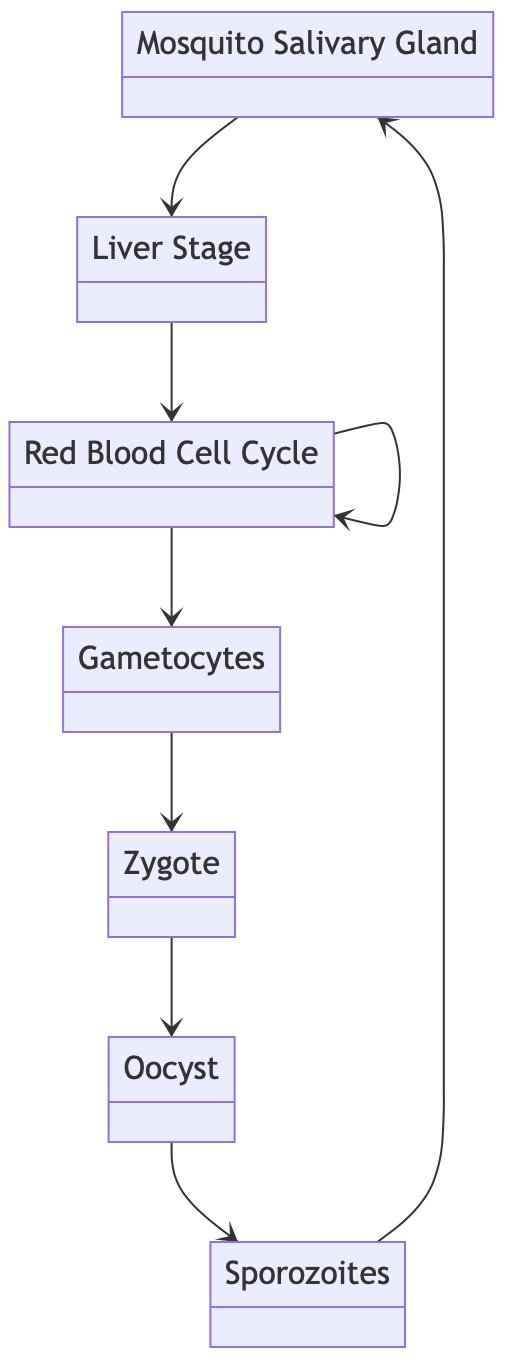
\includegraphics[width=0.4\textwidth]{malaria-life-cycle-diagram}
	\caption{malaria life cycle diagram}
	\label{fig:malaria-life-cycle-diagram}
\end{figure}

\begin{parameter}{\gls{eip}}
	The parasite enters the mosquito during a blood meal, and the mosquito becomes infectious 10-16 days later after the parasite develops into sporozoites.
	The period was called the \gls{eip}.
\end{parameter}

Individual malaria infection can last for many months, during which densities of both asexual parasites and gametocytes vary irregularly as consequences mainly of the parasite's developmental cycle, host immunity, and antigenic variation.
Duration of infection in the model followed convolution of exponential distribution or log-normal distribution or fixed.

\begin{parameter}
	{The length of disease.}
	{Untreated or improperly treated infection last about 200 days on average.
  Some could last for more than a year.}
\end{parameter}

A human host could be in one of the following state:
\begin{itemize}
	\item Susceptible
	\item Treating
	\item Disease(with symptom)
	\item Patently Asymptomatic
	\item Sub-patent stage
	\item Prophylactic protection
\end{itemize}

\begin{figure}[t]
	\centering
	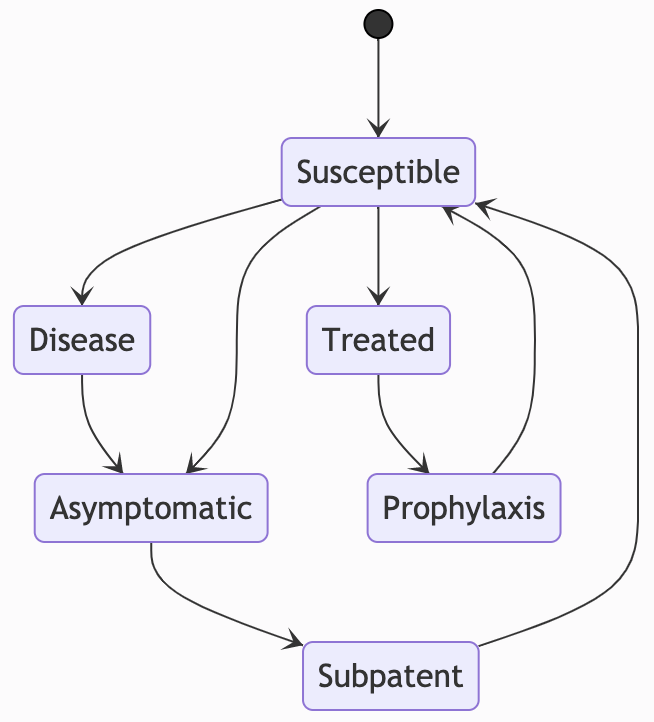
\includegraphics[keepaspectratio=true, scale=0.8]{images/disease-state-transition-diagram.png}
	\label{fig:human_state}
	\caption{Human host disease states transition}
\end{figure}

The rate of state transition decides the trends of the system.
In \ref{fig:human_state}, each arrow denotes a transition from one state to another.
Furthermore, the transition rates vary from each other.
The system will reach an equilibrium after the length of the simulation.

Malaria models from SwissTPH had their core individual humans with vary parasite densities.
The varying level then will affect the possibilities of the state transition.
Infected human will be more likely transit to the next level when they have higher densities.
GSK predicted clinical malaria based on parasite densities using MAP categories for low, moderate, and high transmission.\cite{Hay2004}
Another study separate infected individuals into three different groups(infected high-density parasites with fever, \gls{pvprlm}, infected PCR detectable parasites)\cite{White2018b}, by symptoms, and detectability.

\subsection{Demography}
Demographics of simulated human populations in the models were harmonised with birth cohort, and population sizes.
Imperial's model derived the age structure of the population from the Tanzania's life table in 2010.
While OpenMalaria used a similar distribution, although with a higher mortality in the first year of life.
For GSK, and EMOD DTK a simple geometric distribution was used that provided a close match to other groups.
In all models the total number of simulated individuals was fixed with a non-growing static population for baseline projections.
However, this does not often conform to the population growth rate in \gls{ssa}.
Due to the similarity of \gls{ssa} population structure, models used truncated exponential distribution with a max age to simulate an age structure in studies\cite{White2018b}.

\subsubsection{Age}
\improvement{TODO: Of xx papers, xx stratified individuals by age}
Due to the strong correlation with body surface area, and the tendency of adults to spend a more significant proportion of time outdoors during the evening, models used age to calculate human biting rates.
Other age-varying factors were adaptive to age.
For example, models usually calculated maternal immunity, and duration of infection \gls{pfpr} at each age groups.
If intervention targeted a specific age group, for example, RTSS, stratification in model output was used to assess different age groups' impact.
The relationship between age, and incidence was compared between models.

Human population data was often lack in some areas.
Some studies estimated the missing data by using data from other similar countries.
The population's age structure is drawn from a statistical distribution(or more specifically, an exponential distribution, due to this type of distribution fits well to \gls{ssa} age structure) from a specific country; for example, Tanzania dataset\cite{Sherrard-Smith2018b} was popular in some studies.
Others\cite{Adimi2010} estimated the age through satellite observations.
The study combined land cover and census in East Africa and generated high-resolution population maps for low-income nations.

\subsubsection{Birth and Death}
Some \gls{abm} models simulated birth and death in population.
Birth was carefully calculated to ensure a constant population\improvement{TODO: add citation}.
However, in \gls{ssa} countries, the stalled decreasing trend of malaria cases may be associated with the growing population.
A universal death rate was introduced to some models \improvement{TODO: add citations} to ensure a constant age distribution.
The death rate was also calculated based on the severity of malaria infection.
\begin{parameter}
	{Human host birth rate:}
	{$b_H$}
\end{parameter}
\begin{parameter}
	{Human host death rate:}
	{$\mu_H$}
\end{parameter}
The new-born children in the model inherited part of mothers' immunity level.
However, this maternal immunity decays over time.
Thus, in the malaria model implementation, the inclusion of birth in the model will decrease the overall average immunity against malaria and make interventions less useful to the disease due to a higher possibility to be infected after an infectious bite.

\subsubsection{Geographic Mobility: move in, and move out of an area}
Increasing human mobility is creating highly favorable conditions for the persistence of diseases being targeted for elimination.
However, host mobility is not a top priority factor for the malaria model.
Models assumed an enclosed area with a constant population for simplification.
That was because, in the high or moderate disease transmission setting, important diseases act as a less significant proportion of total infections.

Nevertheless, in the malaria elimination scenario, imported cases are the most critical threat.
Modeling population flow, in that case, would be helpful for countries in the elimination stage to quantify the threats.
In that case, we need predictive models of human movement to help inform how best to target strategies.

Only a few models\cite{Zhu2015a} considered human mobility.
One study focused on pertinent trip data to the gravity model, and radiation model\cite{Marshall2018}.
The relationships between travel distance, and frequency were studied.
Another model\cite{acevedo_spatial_2015} used the extended Ross-Ronald model to the interplay between spatial transmission heterogeneity, and human mobility and their combined influence on prevalence, and \gls{R0}.
These models may help predict the spatial transmission of malaria parasites, and inform strategies to control their spread.

In contrast to host mobility, vector mobility is rarely included in mathematical models.
Vector mobility may be an essential factor, especially for the impact analysis of invasive vectors such as \textit{An. stephensi}.

\subsection{Immunity}
The dynamics of acquisition, and loss of immunity are key parameters determining the speed of decline in parasite prevalence once the transmission is reduced.
Immunity was depicted as dependent on anti-parasite immunity (AP), and clinical immunity (AC).
The acquisition of both anti-parasite, and clinical immunity is assumed to be age, and exposure-dependent.

In particular, models assumed anti-parasite immunity to have two effects:
\begin{itemize}
	\item reducing the probability that a blood-stage infection will achieve sufficiently high density to be detectable by light microscopy;
	\item increasing the rate at which low-density infections are cleared (rPCR).
\end{itemize}
Acquired immunity alters the likelihood that infection results in clinical disease, modifies onward infectivity to mosquitoes, affects the detectability of infection, and modifies the duration of parasitemia.
Clinical immunity is assumed to reduce the probability that a high-density blood-stage infection will progress to cause a symptomatic episode of clinical malaria.

Immunity could be further dissected into four categories:
\begin{itemize}
	\item  maternal immunity, which protects against clinical disease, is assumed to decay exponentially from birth;
	\item  anti-disease immunity, which reduces the probability of developing clinical symptoms on infection;
	\item infection-blocking immunity;
	\item anti-parasite immunity, help individuals control parasite densities, and leave the patent infection state more quickly
\end{itemize}
Infection-blocking immunity, and anti-parasite immunity are both exposure-driven.
While anti-parasite immunity is assumed to develop with age, conditional on having been exposed.
Griffin et al.\cite{Griffin2010} classified infection-blocking immunity as pre-erythrocytic immunity which will result in the reduction in the probability of establishing infection followed by an infectious challenge.

\subsubsection{Acquisition}%
\label{par:acquisition}
The acquisition of immunity is assumed to be age, and exposure-dependent.
A study\cite{White2018b} assumed that both primary infections, and relapses contribute to acquired immunity, and each new infection will boost immunity.
The boosting level is based on the \gls{foi}, and the refractory period.

\subsubsection{Decay}%
\label{par:decay}
Antibodies against \textit{Plasmodium} decay exponentially over time.

\improvement{TODO: among xx studied paper, xx dictated the rate of decay of immunity level}
Different versions of models describe the rate of immunity decay differently.
Imperial models implemented exponential decay of naturally acquired immunity.

\improvement{TODO: Describe the decay rate mathematically}

Models incorporated immunity level, and affect the probability that infection becomes detectable, and the duration of a blood-stage infection.

\subsubsection{Maternal Immunity}%
\label{subsec:maternal_immunity}
Children will get the maternal antibodies from their mothers.
The model assumed a new-born infant would acquire a fraction of their mothers’ anti-parasite, and clinical immunity.
Individuals begin life susceptible to infection, but with partial maternal immunity determined by the level of immunity in women of childbearing age.
Maternal immunity will protect the new-born infant from infections and will decay exponentially after some time. 
\begin{equation}
	I_{maternal} = e^{- \frac{a}{d_{maternal}}}
\end{equation}

Here,

\begin{parameter}
	{$I_{maternal}$}
	{denotes maternal immunity.}
\end{parameter}
\begin{parameter}
	{$d_{maternal}$}
	{denotes the exponential decay rate of maternal immunity.}
\end{parameter}
\begin{parameter}
	{$a$}
	{denotes the age.}
\end{parameter}

Maternal immunity decays in the first six months of life, thereby increasing susceptibility to disease.

\subsubsection{Anti-infection immunity}
\thiswillnotshow{gai}
Individuals become infected at a rate determined by the \gls{foi} in the population, which is determined by the ratio of vectors to humans, the biting rate per mosquito on humans, the proportion of infectious mosquitoes in the vector population, and the person’s level of \textbf{anti-infection immunity}.

%\paragraph{Acquired immunity}%
%\label{par:acquired_immunity}
%Acquired immunity, including clinical immunity, and \improvement{add another type}.

\section{Vector}%
\label{sec:vector}
Detailed implementation of vector life cycle, and entomology were joint in model implementation.
Mosquito behaviors, such as lifespan, density-dependent larval development, feeding, and resting behavior, feeding habits, movement patterns, and biting frequency, are often modeled in detail.
More models implemented vector dynamics as a stochastic version of the compartmental model\cite{Sherrard-Smith2018b}, but only a few explicitly modeled vectors individually as \gls{abm}. 
Models most commonly assessed the interventions impacting vector mortality, such as \gls{irs}, \gls{itn}, and larval source management.
When models also included a spatial component, malaria transmission generally required vector, and host to be co-located.

\subsection{Gonotrophic Cycle}
Simulations used a ‘decision tree’ to represent the timing of movements, and other necessary actions.
The gonotrophic cycle of a female mosquito begins with a blood meal taken from a host and follows by a period of resting and waiting for digestion.
It may take several blood meals before searching for a breeding site for oviposition.
After egg maturation, the mosquito finds a suitable site, and then lays 80 – 100 eggs.
Then mosquitoes will search for another blood meal, and repeat the gonotrophic cycle.
Larvae emerge from eggs.
After four morphologically larval instars, larvae transform into pupae which develop into adult mosquitoes.
The larval period's duration depends mainly on temperature, lasting 7-15 days in tropical areas.

\begin{figure}[htpb]
	\centering
	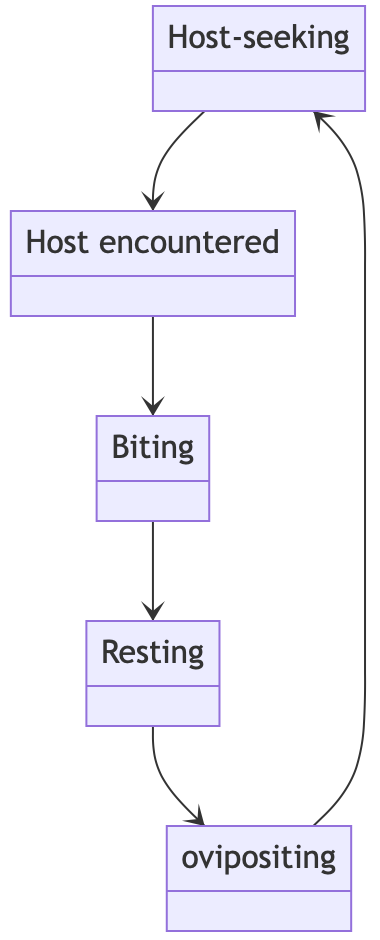
\includegraphics[width=0.4\textwidth]{gonotrophic-cycle-diagram}
	\caption{Gonotrophic cycle diagram}
	\label{fig:gonotrophic-cycle-diagram}
\end{figure}

\subsection{Adult Mosquitoes}
Each adult vector can be in one of three states, susceptible($S$), latently infected(E), and infectious(I).
The number of mosquitoes in susceptible groups will increase as larvae metamorphose into an adult at a rate determined by the birth rate of a specific mosquito species and environment capacity and decrease as susceptible mosquito die at some rate and be infected through a bite from an infected host.
Models use \gls{foi} from human to mosquito to define the rate of mosquitoes' infection rate.
Multiple factors could influence this rate, such as the intervention implemented, and malaria prevalence in the host group.
\begin{equation}
  \frac{dS_M}{dt} = \beta(t) - \Lambda_M S_M - \mu S_M
\end{equation}
where,
\begin{centering}
  $\Lambda_M$ - \gls{foi} from host to vector \\
  $\mu$ - death rate of mosquito\\
  $\beta(t)$ - birth rate at time  $t$\\
\end{centering}

The infected adult mosquitoes then move into the latently infected group.
After an \gls{eip}, these mosquitoes finally move into the infected group.
\begin{align}
  \frac{dE_M}{dt} & = \Lambda_M S_M - \Lambda_M (t- \tau_M) S_M (t - \tau_M) P - \mu E_M\\
  \frac{dI_M}{dt} & = \Lambda_M (t- \tau_M) S_M (t - \tau_M) P - \mu I_M
\end{align}

Where,
\begin{centering}
  $\tau_M$ - \gls{eip} \\
\end{centering}

\subsubsection{Parameters of Adult Mosquitoes in Model Implementation}
\paragraph{Species}%
\label{par:species}
Some studies explicitly toke heterogeneities of different mosquito species into the model.
\textit{An. gambiae} is the dominant species used in most models.
However, different species, including \textit{An. arabiensis}, \textit{An. vagus}, \textit{An. stephensi}, \textit{An. darlingi} were also included in some other models.
Different combinations of species were also common in the implementation.
The host preferential and feeding habits of different species are the most critical factors that affect the intervention effectiveness.
Generally, the lower the proportion of human blood-feeding and night blood feeding, the lower the intervention's efficiency targeted at protection at night, such as \gls{llins}.

Different species vary in entomology indexes.
For example, comparing to \textit{An. gambiae}, \textit{An. arabiensis} has a significantly lower rate in \gls{hbi}.

\paragraph{Endophily}%
\label{par:endophily}
affects residual transmission, and will influence the effect of indoor residual spraying.
Research papers often take endophily as a fixed parameter in the model, which means for each different vector, there is one level of endophily accordingly.

Does endophily change over time or based on the seasons?
In a lower temperature,  some vector species tend to reside in the indoor environment.
However, this variation does not specifically cover in the papers, some studies used seasonal carrying capacity to incorporate the variation.

\paragraph{Parasite density}%
\label{par:parasite_density}
Most studies assumed that all the vectors with salivary gland sporozoites are equally infectious.
The level of infectiousness was expressed as a \gls{foi} from vector to human, calculated as same after the \gls{eip}.

Churcher et al.\cite{Churcher2017a} demonstrated a dose-dependency for the probability of infection.
Vectors with a more significant number of sporozoites have a higher possibility to cause infection.
The heterogeneity in parasite density might be another parameter that could be implemented in other models.

%\improvement{Create a database from research papers to see the different settings of endophily of vector species}
%
%\paragraph{Daily survival rate}
%
%\paragraph{Human visiting rate}
%
%\paragraph{Extrinsic Incubation Period}
%Average incubation period in days
%Extrinsic incubation period
%Features describing a group of vectors (may influenced by interventions)
%The composition of the species of given an area
%The distribution of vectors
%The overall birth rates of vectors
%Types of birth rates defined in the papers
%fixed (constant)
%The distribution of the length of feeding cycle
%Related to species, interventions used
%\improvement{add two figures(using normal distribution)}
%Distribution before intervention
%Distribution after intervention
%
%The distribution of the life span of a given group
%
%\paragraph{Cycling Repeating Rate}
%Cycling repeating rate
%
%\paragraph{Flying ability}
%How long could it fly in a given time
%
%Mathematical function:
%
%A spatial distribution for a given time, e.g.
%
%The ability could determine whether an infectious bite could be transmitted from one to another in a long distance.
%
%\improvement{TODO:
%	Add distribution example
%	Add mathematical function
%	Collect information from papers, and create a database}
%\paragraph{HBI}
%\gls{hbi}
%Related to species, intervention
%Usage of \gls{llins}, and/or \gls{irs} will discourage human biting divert more bites onto non-human hosts
%
%The birth rates may vary in the different settings.
%E.g. `\ ' for a colony of germ in the, the reproduction process follows to a logistic growth:
%\improvement{TODO: added an example figure of logistic growth}
%
%Does the birth rate of vectors follow the same line?
%
%\subsection{Larval}
%Most models only incorporated the adult mosquito part into their implementations.
%Others explicitly modeled the whole larvae living cycle to understand the potential effects of larval source managements.
%
%Based on the entomological  
%Larvae feed on yeasts, bacteria, and organic matter.
%After four molts, larvae become pupae and then develop into adult mosquitoes.
%
%\paragraph{Carrying capacity}%
%\label{par:carrying_capacity}
%\begin{parameter}
%Carrying capacity, describe how many mosquito larvae or pupae an environment can support.
%\end{parameter}
%
%\paragraph{competition}%
%\label{par:competition}
%Two different forms of density-dependent competition in the larval stages:
%
%\begin{itemize}
%	\item contest competition: the number of larvae reaches a limit as initial edge density increases. Due to (i) increased mortality at a higher density (ii) increased developmental time (iii) reduced larval size.
%	\item scramble competition: the number of larvae decreases at higher initial egg density. Due to (i) cannibalism of early instar larvae by late instar, and (ii)increased predators' population .
%\end{itemize}
%
%Environmental larval source management -- reduce carrying capacity.
%
%IRS or LLINs - reduction in oviposition -- reduce density-dependent competition between larvae -- decreased larval mortality
%
%\paragraph{Larval Population Dynamics}%
%\label{par:larval_population_dynamics}
%
%\begin{parameter}
%	\label{para:eggs_laid_per_day}
%
%	Eggs Rate: $\beta$, number of eggs laid per day by each female mosquito.
%	\[
%		\beta=\frac{eggs\:laid\:in\:life\:time}{expected\:life\:time}
%		.\]
%
%\end{parameter}

\subsection{Insecticide Resistance}
Insecticide resistance 
There are multiple mechanisms driving resistance against chemicals in the mosquito population.
Riveron\cite{Riveron2014b} et al. reported the over-expression of detoxification genes as the main driving force of insecticide resistance in \textit{Anopheles} species.

Discriminating dose bioassays (WHO tube assay, WHO cone assay, CDC bottle assay) is a practical option for control programs to assess the mosquito population's proportion killed by a standard dose.
Resistance level in discriminating bioassay was denoted as the percentage of mosquitoes surviving 24-hours following exposure.
Although the simple bioassay has its limitations, it provides a useful measure to link the severity of mosquito insecticide resistance estimated in the field to the results of experimental hut trials evaluating new products.

Mathematical models could help understand the impact of insecticide resistance on malaria control efficiency by (i) making a correlation between resistance level with intervention outcomes; (ii) elaborating the potential evolution and its impact.
A strong association between the level of resistance, and mosquito mortality was observed in the experimental hut trial\cite{Sherrard-Smith2018b}.
Moreover, strong correlation between direct protection against feeding, and the bioassay result was analyzed by Briet et al.\cite{Briet2013}.
Mohammed-Awel et al.\cite{Mohammed-Awel2019} developed a model, simulated the relationship of the usage of interventions, assessing the impact of insecticide resistance in the mosquito population and the frequency of resistant alleles at equilibrium in the community. 
The epidemiology-genetics model couples disease epidemiology with vector population genetics studied the equilibrium state of a deterministic dynamic malaria model and presented the resistance allele dominance associated with the insecticide resistance in the mosquito population.
The study showed that in moderate and high malaria transmission settings, the \gls{itn}-\gls{irs} strategy could lead to the effective control of the disease, but in a more extended simulation, it fails to manage insecticide resistance (as measured in terms of the frequency of resistant allele).
Another study\cite{Gourley2011} compared two mathematical models to understand hot to slow the evolution of insecticide resistance in mosquitoes.
The study concluded a much slower time scale that insecticide-resistant mosquitoes will become dominant if an insecticide targeted at older adult mosquitoes.

\unsure{to understand how they made the connection: did the researcher match the bioassay result to the experimental hut trial data? Find conclusions, and methods in the paper, and summarized it in this document.}
\unsure{how does mosquito resistance affect the repel rate? Why do the mosquitoes don't like the pyrethroid  smell? And why does the mosquitoes' repel rate drops down when the resistance level goes up?}

Therefore overall cost-effectiveness will be lower.  
One comment on the second point is that there is a certain threshold level for the resistance level and active ingredient.
When combining these two factors, we might able to calculate the overall efficacy of the sufficient length.

%\subsubsection{Measurement of Resistance}
%WHO cone test,tunnel test
%release capture test
%
%Bioassay:
%
%\begin{itemize}
%	\item Discriminating Bioassay
%	\item Intensity Bioassay
%	\item Mechanism Bioassay
%	\item Non-standard Bioassay
%\end{itemize}


%\section{Force of Infection, and EIR}%
%\label{sec:force_of_infection_and_eir}

%\subsection{\texorpdfstring{\gls{foi}}{Force of Infection}}%
%\label{sub:foi}

\subsection{\texorpdfstring{\gls{eir}}{EIR}}%
\label{sub:eir}
\gls{eir} is the driving parameter of malaria mathematical models.
Three of the models are driven by \gls{eir} (EMOD DTK, Imperial, and OpenMalaria).
Only a few models use prevalence rather than \gls{eir}as the input.
The relationship between \gls{eir} and intervention outcomes was studied by varying the corresponding \gls{eir} from 0 to 512 infectious bites per person per year.

\section{Interventions}
Interventions could broadly be divided into those targeted at the human host (e.g., pharmacological) or the vector.
Among the variates of intervention, \gls{llins} and \gls{irs} were widely carried out in the malaria endemic countries. 
To analyzed the effects and simulate them in the mathematical modeling, studies summarized their effects in general: when intervention has been applied,

\begin{itemize}
	\item the number of mosquitoes entered compared to those without interventions;
  \item the probability of successfully blood-feeding;
	\item the probability of deterrence from entering, or the number of mosquitoes exit without feeding compared to those without interventions, and;
	\item the mortality rate of mosquitoes exposed to interventions.
\end{itemize}

are explicitly studied and implemented in models.

Models then combine these four probability to calculate the two parameters: 
\begin{itemize}
	\item the level of survival rates dropped for adults mosquitoes in the \gls{eip} and;
	\item the decreased eggs being oviposited in breeding sites.
\end{itemize}

Interventions targeting adult mosquitoes benefit from reducing the probability that an infected mosquito survives sporogony to become infectious, but reduced oviposition will lower larvae's inner competition, reducing larvae mortality.
While interventions targeting larvae will result in a drop in mosquito density, but the proportion of infected mosquitoes will remain the same or even increase(due to the reduced competition in adult mosquitoes for blood meals).

Models further calculate \gls{eir} and \gls{foi} based on them.

Realistic intervention variables, including attrition of LLINs due to wear, and tear, waning of insecticides used within \gls{irs} or \gls{llins}, and a prespecified correlation between interventions, and rounds of the same intervention was included in some models\cite{Walker2016}.

\subsection{\texorpdfstring{\gls{llins}}{LLINs}}%
\label{sub:llins}

\subsubsection{Initial Efficacy}%
\label{subsub:initial_efficacy}

\paragraph{Usage rate}%
\label{par:usage_rate}

Usage rate depicts the proportion of population that use \gls{llins}.
However, studies have different definitions of the rate.
Briët et al.\cite{Briet2013} interpreted as the probability that host searching occurs when people who own a net are using the net.
Under such definition, adults could have a lower usage rate than children.

\paragraph{Interval of simulation}%
\label{par:interval_of_simulation}
The mass campaign is a way to distribute \gls{llins} in \gls{ssa}.
The interval between campaigns is crucial for sustain the effectiveness of nets.
Models used a variety of intervals.
Among which, 2, 3, 4\cite{Walker2016} were the typical alternatives.

Studies showed the declined trend of \gls{llins} effectiveness due to the net's pyrethroid and integrity attrition.
Overall effectiveness will be less influenced by attrition for a short interval.

\paragraph{Initial insecticides}%
\label{par:initial_insecticides}
Some stochastic models explicitly implemented the nets' initial insecticide as it follows a Gaussian distribution.
In \cite{Briet2013}, initial insecticide was set to \SI{55}{mg/m^2}.

%\subsubsection{effectiveness}
%\improvement{TODO: what kind of index studies focused? EIR? DALYs? Prevalence?}
%Studies focused on assessing the impact of malaria transmission interventions , mosquito prevalence, \gls{eir}, cases averted.
%
%Prevalence results from Uganda \gls{rct}\cite{Staedke2020}:
%\begin{center}
%	\begin{tabular}{c c c c}
%    \toprule
%		Type        & 6 months & 12 months & 18 months \\
%    \midrule
%		\gls{llins} & 15       & 13        & 14        \\
%		\gls{pbo}   & 11       & 11        & 12        \\
%    \bottomrule
%	\end{tabular}
%\end{center}

\subsubsection{Distribution}%
\label{sub:distribution}
Studies assumed diverse forms of distribution to reproduce authenticity.
Mass distribution through free distribution campaign was the typical setting.
The interval of mass distribution is vital to the intervention program's overall effectiveness, as the effectiveness decay thorough out time.
Other studies had more comprehensive settings of distribution.
Usage and coverage rates were set as a distribution target.
Before the intervention strategy, the hypothetical area did not reach a certain level of net coverage.
Some studies assumed a gradual increase in the coverage, while other assumed an immediate hight amount level.
For example, in \cite{Griffin2010}, two hypothetical distribution strategies were assumed.
Firstly, the model assumed a gradual increase to 80\% in five years, and a new net to be distributed to individuals every five years.
Secondly, the model further assumed immediate distribution at 80\% coverage, and redistribution every five years.

More flexibility in the distribution strategies would be a welcoming feature for the \gls{nmcp}s as cost-effectiveness, and practicability were crucial for field application.

\subsubsection{Attrition}
\label{subsub:attrition}
Numerous \gls{rct}s and \gls{eht}s proved the attrition of the nets as a significant factor affects the overall intervention effects.
From Tanzania\cite{Protopopoff2018} \gls{rct}, the permethrin, and \gls{pbo} concentration dropped at a steady-rate for both standard \gls{llins}, and Pyrethroid-PBO \gls{llins}:

\begin{center}
	\begin{tabular}{cSSS}
		\toprule
    chemical             & {0 months} & {12 months} & {21 months} \\
		\midrule
		Permethrin (Regular) & 21.4     & 21.5      & 16.7      \\
		Permethrin (PBO)     & 20.9     & 14.7      & 12.2      \\
		PBO                  & 9.5      & 2.9       & 1.6       \\
		\bottomrule
	\end{tabular}
\end{center}

From Uganda\cite{Staedke2020}, the \gls{pbo} dropped:
\begin{center}
	\begin{tabular}{cSS}
		\toprule
    chemical     & {0 months} & {12 months} \\
		\midrule
		PermaNet 3.0 & 26.1    & 15.3    \\
		Olyset Plus  & 8.1     & 5.0      \\
		\bottomrule
	\end{tabular}
\end{center}

Usage attrition from Tanzania\cite{Protopopoff2018}:

\begin{center}
	\begin{tabular}{cSS}
		\toprule
    index     & {4 months} & {21 months} \\
		\midrule
		ownership & 97.6     &           \\
		access    & 89.6     & 70.2      \\
		usage     & 76.9     & 50.6      \\
		\bottomrule
	\end{tabular}
\end{center}

\begin{center}
	\begin{tabular}{cSSS}
		\toprule
    \gls{irs}      & {0 months} & {9 months} & {12 months}\\
    \midrule
		Actellic 300CS & 0.99     & 0.82     & 0.59      \\
    \bottomrule
	\end{tabular}
\end{center}

Usage attrition from Uganda\cite{Staedke2020} showed a much slower trend in the decease in usage:

\begin{center}
	\begin{tabular}{c c c c}
    \toprule
		index             & 6 months & 12 months & 18 months \\
    \midrule
		ownership         & 97       & 95        & 91        \\
		adequate coverage & 71       & 63        & 51        \\
		usage             & 85       & 79        & 73        \\
    \bottomrule
	\end{tabular}
\end{center}

Mathematical studies described the attrition of \gls{llins} as the composition of insecticide decay, and impairment of physical integrity.
The effectiveness of \gls{llins} will discount with the attrition of nets.

\paragraph{Physical integrity}
Information on durability of physical integrity of LLINs and community usage is essential to maintain optimal coverage for an effective and sustainable malaria control strategy.
Studies dissected physical integrity into two factors:

\subparagraph{Hole rate}%
\label{par:hole_rate}
The level of the annual hole formation rate of nets.
This rate was set at 1.8 holes per net per year in \cite{Briet2013}.
For the stochastic model, heterogeneity is essential for modeling.
The model would vary the hole rate by multiplying a distribution factor, e.g. Briet et al. \cite{Briet2013} assumed the hole rate follows a log-normal distribution.

\subparagraph{Rip rate}%
\label{par:rip_rate}
A net’s hole index is the hole count plus the rip factor value multiplied with the cumulative number of rips.

\paragraph{Half-life}
\label{par:half_life}

Some studies explicitly defined the attrition of nets by using the concept of `half-life'.
The definition implied exponential decay rate of the effectiveness.
However, the definition of half-life in \gls{llins} varies in studies.

\begin{table}[htpb]
  \centering
  \caption{Different settings for \gls{llins} in models}
  \label{tab:different_settings_for_llins}
  \begin{tabular}{cS}
  \toprule
  study & {half-life} \\
  \midrule
  \cite{Briet2013} & 4 \\
  \cite{Griffin2010} & 2.64 \\
  \bottomrule
  \end{tabular}
\end{table}

In \cite{Briet2013}, the half-life was described as diminishing in net number after a single mass distribution.

\begin{equation}
  \phi(t) = e^{- \frac{t}{L} }
\end{equation}
\begin{center}
  L - parameter for exponential decay rate
\end{center}

The model then combines the half-life index(attrition of number) with the decayed insecticide, and physical integrity to calculate diminishing effects on control.
In \cite{Griffin2010}, the half-life was defined to describe the decay rate of the nets' protective efficacy due to decaying insecticide efficacy, and wear-and-tear.
Under such definition, the half-life was the index that combines insecticide decay and physical deterioration.

However, a single half-life of the nets can not express real-world heterogeneity due to the varying environment and the different washing net habits.
Thus, heterogeneity in stochastic model could further simulate these effects by assuming the half-life or decay rate follows a statistical distribution(often a Gaussian distribution).
The variation in insecticide and physical integrity will increase over time under such a setting due to the decay rate's heterogeneity.

%From the \gls{rct}s dataset, 
\subsection{PBO}
\gls{pbo} is a synergist targeting oxidate-based pyrethroid resistance in \textit{Anopheles} species.
It provides an alternate choice for field control.
\gls{eht}\cite{Akoton2018a}, and \gls{rct}s proved to be more effective on resistant, and/or multi-resistant mosquito populations.
\improvement{TODO: add refs}

Some studies made assumptions of statistical correlations between insecticides' effectiveness with and without PBO:

\begin{align}
  PBO & = \alpha_p + \lambda_p \frac{((1-\beta) - 0.5)}{1 + \gamma_p ((1-\beta) - 0.5)} \\
  \gamma_a & = \frac{e^{PBO}}{1 + e^{PBO}}\\
  \gamma_a & = 1 - \beta\\
  \gamma_h' & = \alpha_h + \lambda_h ( \gamma_a - 0.5 ) \\ 
  \gamma_h & = \frac{e_{\gamma_h'}}{1+e^{\gamma_h'}}
\end{align}



\subsection{\texorpdfstring{\gls{irs}}{IRS}}
\gls{irs} is an integral part of malaria control.
Mathematical models considered the following factors and varying parameters of \gls{irs}\cite{Sherrard-Smith2018b}:

\begin{itemize}
	\item Initial efficacy on mosquito populations. The ability to kill or deter mosquitoes from entering a sprayed structure. Models denote the efficacy as the probability of successful blood feeding, mortality rate when mosquito rest on the sprayed surfaces, and deterrence rate;
	\item impact duration (the residual half-life);
  \item Insecticide gradients, and their difference in efficacy;
	\item where, and when sprays are deployed (local malaria endemicity, timing of applying, seasonality of transmission, mosquito species, human behavior, and net-use);
	\item spray quality coverage and; 
  \item the cost, and cost-effectiveness of \gls{irs}.
\end{itemize}

Among these factors, the first point, or product-induced vector mortality, blood-feeding inhibition, exophily, and deterrence were significantly statistically studied, and considered vital indicators due to the accessibility of \gls{eht} data.
These four indicators were explicitly considered the starting point to assess \gls{irs}'s efficacy in malaria control and were modeled in the comparative studies.

Along with initial efficacy, models also put emphasis on the impact duration due to the \gls{irs} relative shorter effective duration comparing to \gls{llins}.
The temporal characteristic of \gls{irs} was studied by fitting it to the \gls{eht} dataset.
Factors including:
\begin{itemize}
  \item Type of wall surface: cement, mud, wood, concretes;
  \item Application location: walls, ceiling, both;
  \item Does \gls{llins} also applied in the area?
  \item Mosquito species;
  \item Active ingredient of \gls{irs}.
\end{itemize}

Some studies also focus on comparing the differences in insecticide gradients.
Four insecticide gradients, pyrethroids (including deltamethrin, lambda-cyhalothrin, and alpha-cypermethrin), are the main insecticides used by \gls{nmcp} for \gls{irs}.
Substantial variation in the initial efficacy of active ingredients was summarized in the study \cite{Sherrard-Smith2018b}.

\subsection{Experimental Hut Trail}
\gls{eht} studies typically report 24h product induced: mortality, blood-feeding inhibition, exophily, and deterrence.
The studies also report the detailed number of female mosquitoes in one of the four states: unfed alive (UA), unfed dead (UD), fed alive (FA), or fed dead (FD).

Modeling calculate these outcomes based on the following formulas:

\begin{parameter}
	\label{eht:mortality}

	Mortality: The number of female mosquitoes found in the hut which are dead on collection or die within the next 24-h.
    \begin{equation}
		Mortality = \frac{D}{N}
    \end{equation}
\end{parameter}


\begin{parameter}
	\label{eht:exophily}
	Exophily: the number of female mosquitoes in exit traps (E) compared to the sum of the number collected in the hut, and exit traps (N).
    \begin{equation}
		Exophily = \frac{E}{N}
    \end{equation}
\end{parameter}

\begin{parameter}
	\label{eht:blood_fed}
	Blood feeding: The number of blood-fed mosquitoes which were collected in the hut, and exit traps.
  \begin{equation}
		BloodFed = \frac{B}{N}
  \end{equation}
\end{parameter}

\begin{parameter}
	\label{eht:Deterrence}
	Deterrence: Reduction in the entry rate of mosquitoes into experimental huts with or without.
  \begin{equation}
		Deterrency = \frac{N_C - N_T}{N_C}
  \end{equation}
\end{parameter}

Explanatory factors:

\begin{parameter}
	\label{eht:experimental_hut_types}
	Experimental hut types: West or East African design
\end{parameter}

\begin{parameter}
	\label{eht:wall_substrate} Wall substrate: Cement or mud
\end{parameter}

\begin{parameter}
	\label{eht:chemical_class_used}
	Chemical types used in \gls{eht}.

	For IRS: carbamate, clothianidin, organophosphate, and pyrethroid

	For LLINs:
	\improvement{TODO: list the chemical class used in the LLINs}

\end{parameter}

Prediction of \gls{eht} outcomes using explanatory factors, combining linear algebra, and non-linear transformation\cite{Sherrard-Smith2018b}:

\[
	\pi_i = logit^{-1} \frac{\ln \pi_i}{1-\pi_i} = \frac{ \exp( \beta + \sum_h \beta_h X^{hi} ) }{ 1 - \exp( \beta + \sum_h \beta_h X^{hi} ) }
	.\]

$\beta_h X^{hi}$ denotes explanatory factors times covarite, which is the hypothetical explanatory space's linear transformation.
The middle part of the formulation then projects $\mathbb{R} \twoheadrightarrow (0,1)$.

\section{Environmental Factors}%
\label{sec:environments}
Core environmental aspects related to vector activity were included, such as water sources for oviposition (egg-laying)\cite{Bomblies2008}, houses for blood meal locations\cite{Gu2009a}, and meteorological data to account for seasonal patterns in transmission\cite{Depinay2004}.
Rainfall, and temperature data were regularly used; model questions included the impact of wet season lengths\cite{Endo2016a}, and hysteresis\cite{Yamana2017} on vector populations.
Environmental factors such as temperature, rainfall, and vegetation density\cite{Gomez-Elipe2007} at different times were incorporated in some models.
Another model create a concepts of environmental carrying capacity.
It is described as how many mosquito larvae or pupae an environment can support due to \gls{isc}. 
Two different forms of density-dependent competition in the larval stages:
\begin{itemize}
	\item contest competition: the number of larvae reaches a limit as initial edge density increases. Due to (i) increased mortality at a higher density (ii) increased developmental time (iii) reduced larval size.
	\item scramble competition: the number of larvae decreases at higher initial egg density. Due to (i) cannibalism of early instar larvae by late instar, and (ii)increased predators' population .
\end{itemize}
\paragraph{Carrying capacity}%
\label{par:carrying_capacity}

\begin{parameter}
Carrying capacity, describe how many mosquito larvae or pupae an environment can support.
\end{parameter}

The \gls{isc} will also affect eggs laid per day.
\begin{parameter}
	\label{para:eggs_laid_per_day}
	Eggs Rate: $\beta$, number of eggs laid per day by each female mosquito.
  \begin{equation}
		\beta=\frac{eggs\:laid\:in\:life\:time}{expected\:life\:time}
  \end{equation}
\end{parameter}

\begin{parameter}
	{Average eggs lay by female \textit{Anopheles}}
	80 - 100 eggs.
\end{parameter}

\begin{parameter}
	{Duration of the larval period}
	Depends on temperature; in tropical areas last 7 - 15 days.\cite{bayoh_lindsay_2003}
\end{parameter}

\begin{parameter}
	{Carrying capacity in aquatic stage}
	Describe how many mosquito larvae/pupae an environment can support
\end{parameter}

%
%\paragraph{competition}%
%\label{par:competition}
%Two different forms of density-dependent competition in the larval stages:
%
%\begin{itemize}
%	\item contest competition: the number of larvae reaches a limit as initial edge density increases. Due to (i) increased mortality at a higher density (ii) increased developmental time (iii) reduced larval size.
%	\item scramble competition: the number of larvae decreases at higher initial egg density. Due to (i) cannibalism of early instar larvae by late instar, and (ii)increased predators' population .
%\end{itemize}
%
%Environmental larval source management -- reduce carrying capacity.
%
%IRS or LLINs - reduction in oviposition -- reduce density-dependent competition between larvae -- decreased larval mortality

\section{Model Output}%
\label{sec:model_output}

Malaria mathematical models are focus the public health outcomes and entomology indexes under different intervention strategies.
Generally, the models’ output include:
\begin{itemize}
	\item The number of clinical cases and number of cases averted;
	\item The number of severe cases, and hospitalized;
  \item \gls{pfpr}\cite{Penny2016} by specified age group; 
  \item \gls{pvprlm}, the prevalence of infection defined by microscopy;
	\item The number of death due to malaria;
  \item Anemia prevalence in specified age group;
	\item \gls{dalys}, and;
	\item Cost-effectiveness.
\end{itemize}
Comparison between baseline settings, and the outcome was conducted to understand the effects on interventions.

\subsection{\texorpdfstring{\gls{dalys} calculation}{DALYs Calculation}}%
\label{sub:dalys_calcualtion}
\gls{dalys} were calculated based on the duration of disability, and respective disability weights.
Weights by disease outcome, and treatment have been obtained from the Global Burden of Disease Life-time disability is assumed for severe episodes that result in neurological sequelae.
Years of life lost (YLLs), and \gls{dalys} were calculated based on the countries' life-table from and assuming an age-specific life expectancies. 
YLLs, and \gls{dalys} were estimated based on a comprehensive measure of deaths, including direct malaria deaths and deaths due to malaria co-morbidities.
While some models only focus on mobility based on direct malaria deaths.

\subsection{Cost Effectiveness}%
\label{sub:cost_effectiveness}
\gls{icers} were the main index for comparing cost-effectiveness.
For example, \gls{icers} was compared between four models in one study to analysis the cost-effectiveness of \gls{rts} \cite{Hay2004}.

\subsubsection{Costs}
Cost of interventions increases when coverage increase.\cite{Winskill2017a} considered two approaches to simulate the function:

\begin{itemize}
	\item linear increases in cost associated with increasing coverage
	\item delivery cost increases logarithmically with increasing coverage
\end{itemize}

Total cost was assumed to consist of two components: the commodity, and the delivery. The commodity part of cost follows U-shape curves follows the marginal cost formula.

\begin{equation}
MC = \frac{\Delta C}{\Delta Q}
\end{equation}

In the short run, marginal cost ($MC$) drops when quantity($Q$) increases, then increases as $Q$ increases.

%\begin{table}[htpb]
%	\centering
%	\caption{Cost of Malaria Interventions}
%	\label{tab:cost_of_malaria_interventions}
%	{\small
%		\begin{tabular}{cSSSSSSSS}
%			\toprule
%			Studies           & {year} & {distributing \gls{llins}} & {\gls{irs}(per person per year)} & {three rounds of seasonal Chemoprevention(per child per year) } & {Non-drug cost of mass screen, and treatment (per person per round)} & {Non-drug cost of mass drug administration (per person per round) } & {Full course of dihydroartemisin-piperaquine} & {Treatment of uncomplicated malaria with artemether-lumefantrine} \\
%			\midrule
%			\cite{Walker2016} & 2016   & 7.03                       & 8.80                             & 5.25                                                            & 5.63                                                                & 2.98                                                                & 1.65                                          & 2.50                                                              \\
%			\bottomrule
%		\end{tabular}
%	}
%\end{table}

\paragraph{\texorpdfstring{\gls{llins}}{LLINs}}
Review from fields was used to estimate the median unit procurement cost, and the delivering cost of \gls{llins}.
The inflation rate calculator was also included in some studies\cite{Walker2016}.

\begin{table}[htpb]
	\centering
	\caption{Cost of \gls{llins}}
	\label{tab:cost_of_llins}
	\begin{tabular}{cSSSS}
		\toprule
		studies           & {year} & {procurement} & {delivering} & {total} \\
		\midrule
		\cite{Walker2016} & 2016   & 5.00          & 1.58         & 7.03    \\
		\bottomrule
	\end{tabular}
\end{table}

\paragraph{\texorpdfstring{\gls{irs}}{IRS}}
Range from USDA 2–3 to roughly USDA 20 per unit\cite{Oxborough2016}
(a unit is standardized across products to cover approximately 250 of wall surface)

\begin{table}[htpb]
	\centering
	\caption{Cost of \gls{irs}}
	\label{tab:cost_of_irs}
	\begin{tabular}{cSSSS}
		\toprule
		studies           & {year} & {procurement} & {delivering} & {total} \\
		\midrule
		\cite{Walker2016} & 2012   &               &              & 8.08    \\
		\bottomrule
	\end{tabular}
\end{table}

%Perennial, and seasonal settings were two concepts describing the seasonal feature in sub-Saharan region.

\paragraph{\texorpdfstring{\gls{rts}}{RTS}}%
\label{sub:rts}
One study\cite{Hay2004} calculated costs of vaccine introduction from the provider perspective but are limited to the cost of consumables, including vaccines, injection and reconstitution syringes, and safety boxes.
Prices are scaled up to account for freight\cite{Winskill2017a}, and wastage\cite{Hutton2006}.

\chapter{Optimization and Evaluation}
\section{Optimization}
\subsection{Parameter Optimization}
\subsubsection{Sources}%
The methods for estimating key parameters varied considerably across the literature.
Most models used past literature or simulations to determine baseline parameter values.
Due to specific inputs' nature, many parameters cannot or have not been estimated in field studies, and consequently, authors used expert knowledge to select these values.

\subsubsection{Calibration}%
\label{par:calibration}
Parameter justification was not always clear\cite{Gurarie2007,Arifin2011a,NiazArifin2013}; when explained, models generally calibrated a range of parameters to existing data or provided references for their choice of fixed values.
Studies used models that were either previously calibrated to data or presented calibration as a component of their work.
Calibration techniques included the use of calibration vectors, least-squares, maximum likelihood functions, and visual estimations.
Bayesian techniques for model fitting could provide credible intervals alongside point estimates of parameters.
Calibrating all model parameters to data is not implemented by most researchers, which necessarily excludes certain parameter combinations that could produce accurate calibrations.
Further, no previous models have calibrated all parameters to data.

\subsubsection{Equilibrium state}%
\label{par:equilibrium_state}
The malaria mathematical modeling also takes the advantage of equilibrium state to estimate the parameters\cite{Alves2021}.
Static models assume the system has reached a steady state solution that does not change with time.
Static models are simpler to formulate, and analyze.
Dynamic models study the evolution of a system over time.
Dynamic models can be either deterministic or stochastic; each version could lead to equilibrium points.
Studies calibrate part of a parameter set by assuming the region has reached the equilibrium state.

\subsubsection{The Total Length of Model Simulation}
3-4 years of length is a typical length for simulating the effectiveness of \gls{llins}.
However, like 20 years, the longer length was used in some studies to understand longer-term effectiveness\cite{Walker2016}.
%\improvement{TODO: an overview of length of model simulation}

\subsubsection{The Length of Time Step in Model Simulation}%
\label{subsub:time_step}
Dynamic models may treat time as discrete units, leading to difference equations, or they may consider continuous-time, leading to differential equations.
There were also considerations relating to the method of agent simulation, and the size of the time step.
Daily time steps were most common.
A temporal resolution of 1-5 days was sufficient to remark the changing disease characteristics.
If the model explicitly incorporated agent actions, more granular time steps are needed.
Hourly status updates were most common, and some models even tracked vectors as frequently as each second.



\subsection{Increasing Clarity}%
\label{sub:incresing_clarity}
Increasing clarity in model reporting would greatly benefit both the creators of models, and their audience.
While many papers included detailed supplementary materials for additional results, project descriptions, and calibration, validation, sensitivity analysis, and optimization techniques, these techniques' intricacies often unclear.
To make model descriptions more understandable, and complete, thereby making \gls{abm} less subject to criticism for being irreproducible, a protocol called \gls{odd} \cite{Grimm2010} was published in 2006 to standardize the published descriptions of \gls{abm}.
Some models that used it \cite{Zhu2015, Zhu2015a, Watson2017} were simple to understand, and appeared easily replicable by external groups.
Further transparency includes sharing of the mathematics, and code{Watson2017} of models.
These small steps in the documentation would allow for increased verification, and validation of models, and increase opportunities for collaboration between modeling groups.

\section{Validation and Evaluation}
Accurate predictions of malaria can provide public health, and clinical health services with the information needed to implement prevention and control measures strategically.
Many \gls{abm} had an emphasis on informing policy, and explicitly aimed to understand specific programmatic questions.
To reliably inform public health decisions, there must be confidence in the assumptions guiding model creation, in particular regarding choice of parameter values.
If modeling groups consider extending their model frameworks significantly to influence policy, evaluation and validation against real-world data are necessary.

\subsection{Model Validation}%
\label{par:validation}
Some models performed model validation.
All major model frameworks were reported as validated.
However, validation techniques were rarely explained in detail.
When described, validation was most commonly performed by running a calibrated simulation and comparing model outputs to a dataset not used for calibration.
Methods like root mean squared error, and absolute difference\cite{Adimi2010, Rahman2011}, 95\% CI(for predicted value, and compared to observed)\cite{Chatterjee2009,Gomez-Elipe2007,Roy2011}, average percentage error\cite{Haghdoost2008}, T-test\cite{Xiao2010}, coefficient correlation\cite{Yacob1947} were used.
For example, validation against \gls{rct} or \gls{eht}.
A typical approach for dealing with data validation was to segment data into a model building or training portion with one other portion(the 'holdout' sample) used for model validation or assessing forecast accuracy.
Studies\cite{Parveen2021,Rahman2011} implemented these methods to perform model validation.
The studies divided raw data into training, and testing groups by excluding the last year of data, then fit the remaining data.
The studies then estimated the accuracy of the predictions from the prediction residuals.
In machine learning studies, data were separated into three groups: the training group, the cross-validation group, and the testing group to prevent overfitting.
The model will fit the parameters using the training group, adjust them by comparing metrics against cross-validation groups, and validate the testing group's final model performance.
Some studies concluded that their model did not accurately fit the data used for validation, suggesting incomplete data may explain any discrepancies.

\subsection{Performance Metrics}%
\label{par:performance_metrics}
The diversity in forecasting accuracy measures, and scale-dependent measures limits the comparability of forecasting results, making it challenging to identify the optimal predictors, and methods for malaria forecasting.
Methods like Akaike’s information criterion, Bayesian information criterion, the coefficient of determination, mean absolute error least-squares estimation for regression models, classification accuracy, the \gls{auc}, F1 score, general Gauss-Markov theorem for classification models were used to choose the best fit model parameters.
%to identify, and assess methods, including predictors, used to forecast malaria is important for 
%\subsubsection{Classification metric}
%\paragraph{Classification accuracy}%
%\label{par:classification_accuracy}
%This is the ratio of the total number of accurate predictions to the total number of input samples used.
%\begin{equation}
%	Accuracy = \frac{Accurate predictions}{Total Predictions}
%\end{equation}
%
%\paragraph{\gls{auc}}%
%\label{par:auc}
%\gls{auc} is used for evaluating binary classification problems.
%\gls{auc} score provides a good summary of the performance of the receiver operator curves.
%The Receiver Operating Characteristics(ROC) curve was plotted between the false-positive rate (FPR), and true-positive rate (TPR), representing the model’s performance, and then the \gls{auc} score was calculated.
%
%\paragraph{F1 score}%
%\label{par:f1_score}
%
%\paragraph{Akaike's information criterion}%
%\label{par:akaike_s_information_criterion}
%
%\subsubsection{Regression metric}
%\paragraph{Least-squares estimation}%
%\label{par:least_squares_estimation}
%R code for least squares estimation calculation:
%\begin{minted}
%{R}
%SIR_SSQ <- function(parameters, dat) {  
%    result <- as.data.frame(ode(  y = initial_state_values # named vector 
%                            , times = times                # vector of times
%                            ,  func = SIR_fn               # SIR function
%                            , parms = parameters)
%    )
%
%    # assumes the data you are fitting to has a column "I"
%    dat <- na.omit(dat) # within the function, 
%                        #select complete cases only from dat
%
%    #select from result$I where the times match the times in the data  
%    deltas2 <- (result$I[result$time %in% dat$time] - dat$I)^2   
%    SSQ   <- sum(deltas2)
%    return(SSQ)
%    }
%\end{minted}
%
%\paragraph{general Gauss-Markov theorem}%
%\label{par:general_gauss_markov_theorem}
%Study\cite{Chatterjee2009} applied this theorem to estimate the confidence intervals for each data points and determine the degree of confidence to be entrusted for model predictions.

\subsection{Comparing to Randomized Control Trials}
Transmission models provide a means of converting entomological measures of efficacy into predicting impacts on public health.
\gls{rct} is the gold standard for assessing intervention efficacy, and effectiveness in the field.
\gls{rct} results were compared to the model predictions by modelers to determine whether parameterizations satisfactorily match the observed data\cite{Sherrard-Smith2018b}.
Models for assessing can generate mean, as well as maximum, and minimum impact.
The parameter sets could be fitted to different \gls{eht}, and then compare the results from \gls{eht}.
Study{Sherrard-Smith2018b} compared the model prediction with the best fit model to two \gls{rct}s.
The predicted prevalence was visually compared to the actual data.

When comparing to the real-world \gls{rct} dataset, uncertainty is crucial.
Generally, a narrower range of uncertainty is considered better.
Part of the uncertainty was caused by natural stochasticity, thus not possible to reduce.
Analysis, and decomposition of the uncertainty level might be essential us to understand the model output.

%\subsection{Cross Comparing}
%
%\subsection{Predict Future Results}

\subsection{Comparing to Different Models}%
\label{par:comparing_models}
Methods of comparing models to data were rarely explained.
Some models outlined methods using log-likelihoods, square distance function, and docking techniques.
Successful model validation was often used to justify extending a model framework to include interventions or assess their potential impact in interest location.
Direct comparison of methods would be easier if multiple malaria forecasting methods were applied to the same data.
It would be helpful if we develop a standard dataset, and standard index for model comparison.

%\begin{table}[htpb]
%	\centering
%	\caption{Model Heterogeneity Comparison}
%	\label{tab:model_heterogeneity_comparison}
%	\begin{tabular}{cc}
%		\toprule
%		model             & \\
%		\midrule
%		\cite{White2018b} & \\
%		\bottomrule
%	\end{tabular}
%\end{table}

\subsection{Intervention Optimization}
Several papers\cite{Tchoumi2020,Smith2008,Cameron2015,Winskill2019} conducted optimization analysis of interventions.
Methods included changing the location, timing, or combination of interventions.
Study use Pontryagin’s Maximum Principle\cite{Tchoumi2020} concerning a time-dependent constant to derive the necessary conditions for the optimal usage of interventions.
Other study use non-linear optimization methods\cite{Walker2016} to examine how optimum packages vary when control measures are deployed, and assessed at national, subnational spatial scales.
A study showed a more granular national malaria control program will result in better cost-effectiveness\cite{Walker2016}.

\subsection{Sensitivity analysis}%
\label{par:sensitivity_analysis}
Some studies\cite{Briet2013,Mohammed-Awel2019, White2018b} explicitly mentioned sensitivity analysis or described parameter variation, and comparison of outputs.
The techniques used were generally informal, with methods used rarely explained in detail, and reporting of results was uncommon.
Where sensitivity analysis was explained, it involved altering calibrated baseline parameter values by a fixed percentage, and assessing changes to the response function.
Speed of loss rate of \gls{llins} adherence\cite{White2018b}\ldots was studies by the sensitivity analysis.
Relationships between population, intervention coverage, \gls{eir}, \gls{llins} type with episodes averted, and \gls{dalys} were analyzed in \cite{Briet2013}.
Formal techniques employed included Latin Hypercube sampling, regression tree analysis, and one-way, and probabilistic sensitivity analysis.

\begin{figure}[htpb]
	\centering
	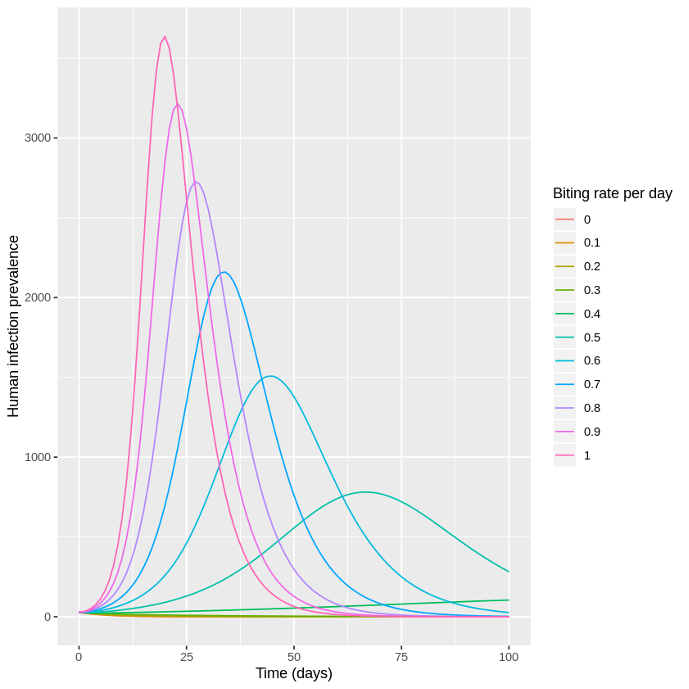
\includegraphics[width=\textwidth]{ross-mcdonald-sensitivity}
	\caption{An example of Sensitivity Analysis with Ross-McDonald Model}
	\label{fig:ross-mcdonald-sensitivity}
\end{figure}
%\section{Method}%
%\label{sec:method}
%\subsection{Search strategy and selection criteria}
%A literature review was performed.
%Database searches of Google Scholar were performed.
%Terms relating to malaria, mathematical model, epidemiology, demography, agent-based, individual-based, microsimulation models were included. No limits were placed on publication type, language, location, dates or publication status.
%
%\section{results}%
%\label{sec:results}
%The search yielded 212 abstracts potentially meeting the inclusion criteria.
%
%\begin{table}
%	\centering
%	\label{tab:overview_of_the_review}
%	\begin{tabular}{c S}
%		\toprule
%		type             & {number} \\
%		\midrule
%		inclusion        & 212      \\
%		full-text review & 50       \\
%		\bottomrule
%	\end{tabular}
%	\caption{Overview of the review}
%\end{table}

\newpage
% appendix
\appendix
\bibliographystyle{unsrt}
\bibliography{library}

\end{document}
